
\section{Setup}

The study was carried out in a room of the GlobIS group. The participants were sitting in front of a 27-inch screen with a 2560x1280 and had access to an English (US) keyboard and a mouse. They also had access to two real devices: A Nexus 7 and an HTC M9. Furthermore, they were given a tutorial sheet about Javascript that contained some functions that are useful for DOM modification as well as arrays. During the study, the instructor was sitting next to the participants and was available to answer any questions that occurred during the study. 

\subsection{Participants}

We recruited 12 participants that all were university members in the department of computer science at ETH Zurich. Most participants were either PhD or Master students, but there were also some Bachelor students. It was required that all participants have at least basic knowledge about front-end web technologies (i.e. HTML, CSS, Javascript). The age of the participants ranged from 23 to 33 and the median age was 26. 

\subsubsection{Previous Experience}
We asked all participants about their previous experience with web application development and Javascript in particular, as well as about their previous experience with responsive web applications and cross-device web applications. Furthermore, we asked them about whether they have used Chrome DevTools before and how they used them. The participants rated their skills in web application development and Javascript on a 5-point Likert scale (see Figure ~\ref{fig:xp}) from basic to proficient and also gave the numbers of years in experience (see Figure ~\ref{fig:years_of_xp}) that they had in web application development and Javascript.

\begin{figure}[H]
  \centering
    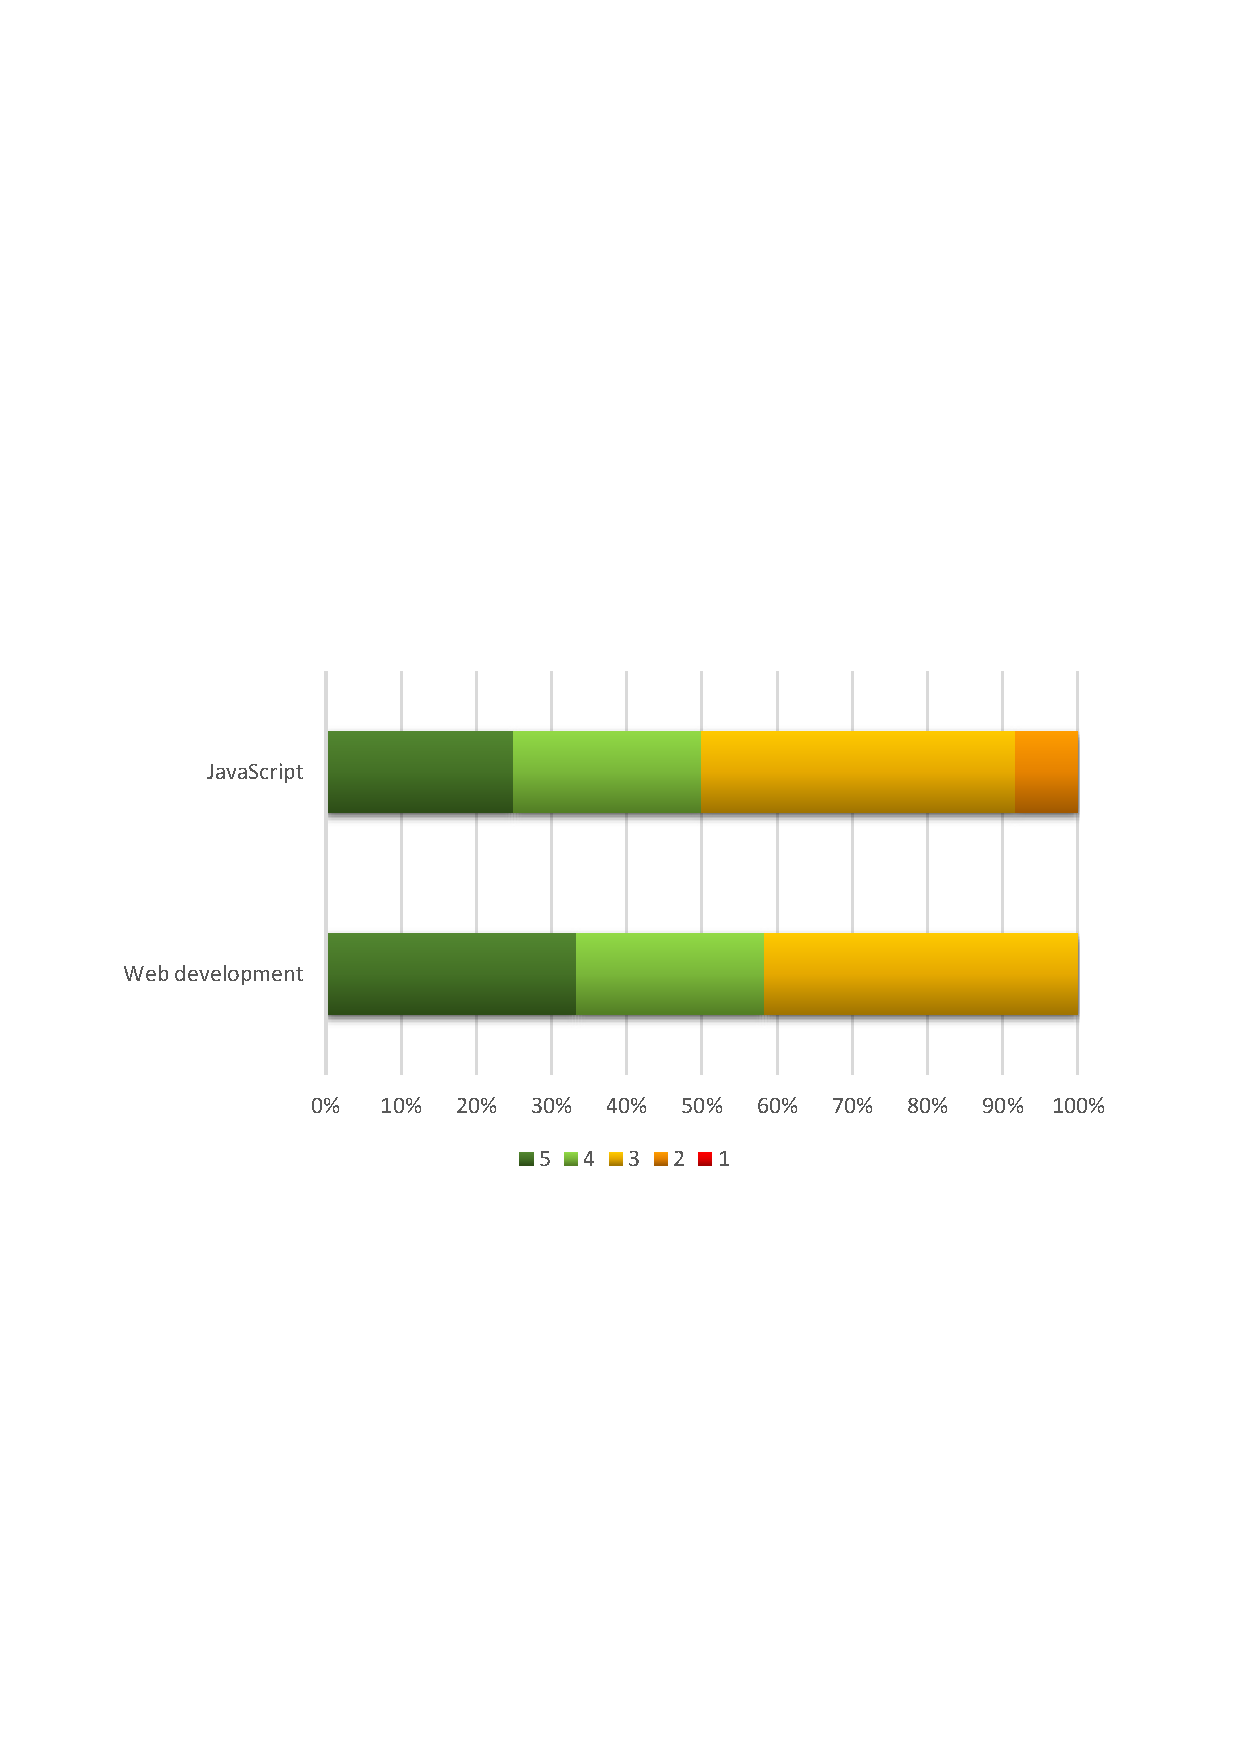
\includegraphics[width=0.8\textwidth]{images/charts/xp.pdf}
	\caption{Previous experience}
	\label{fig:xp}
\end{figure}

\begin{figure}[H]
  \centering
    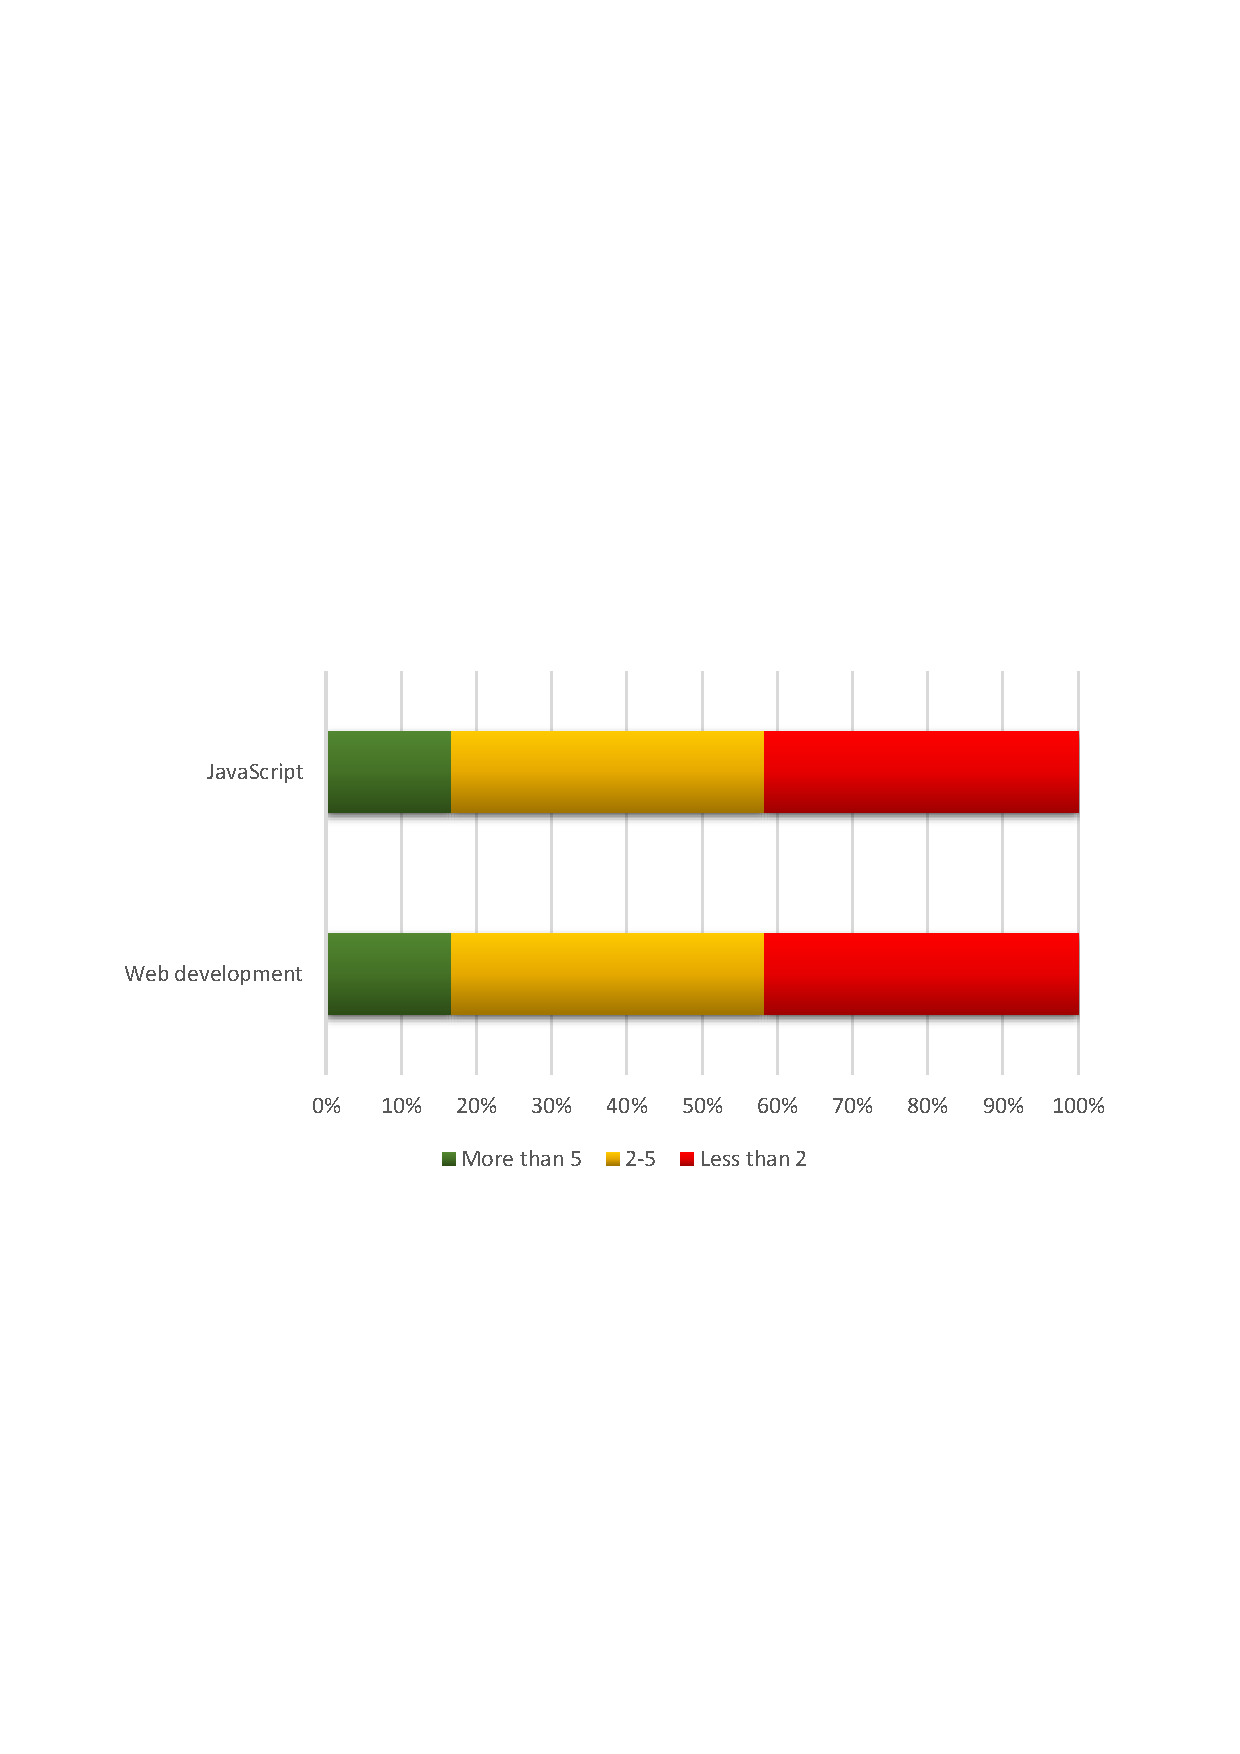
\includegraphics[width=0.8\textwidth]{images/charts/years_of_xp.pdf}
	\caption{Years of experience}
	\label{fig:years_of_xp}
\end{figure}

Eight out of the twelve participants stated that they already had some experience with developing responsive web applications. All of them either used browser tools for emulating devices to test their applications or real devices. Some also used both.

Seven participants already had some experiences with cross-device application development. Again, most of them used browser tools for emulating devices or real devices for testing their applications. Four of them either used multiple browsers, multiple browser profiles or incognito modes to simulate multiple devices on one device. Thus, about half of the participants that already had some cross-device experience constantly used multiple devices to test their applications.

Most of the participants already had experience with Chrome DevTools, only three participants indicated that they had never used them before. We asked participants how often they used certain features of Chrome DevTools, in particular Device Mode, HTML and CSS inspection, Javascript debugging and the console (see Figure ~\ref{fig:devtools_xp}). Device Mode was rarely used by the participants, which is no surprise, given that it is a rather new feature. All participants stated that they often use HTML and CSS inspection, thus this seems to be the most popular feature. The console was also used rather often. Surprisingly, Javascript debugging was not that popular, less than half of the participants stated that they often use it.

\begin{figure}[H]
  \centering
    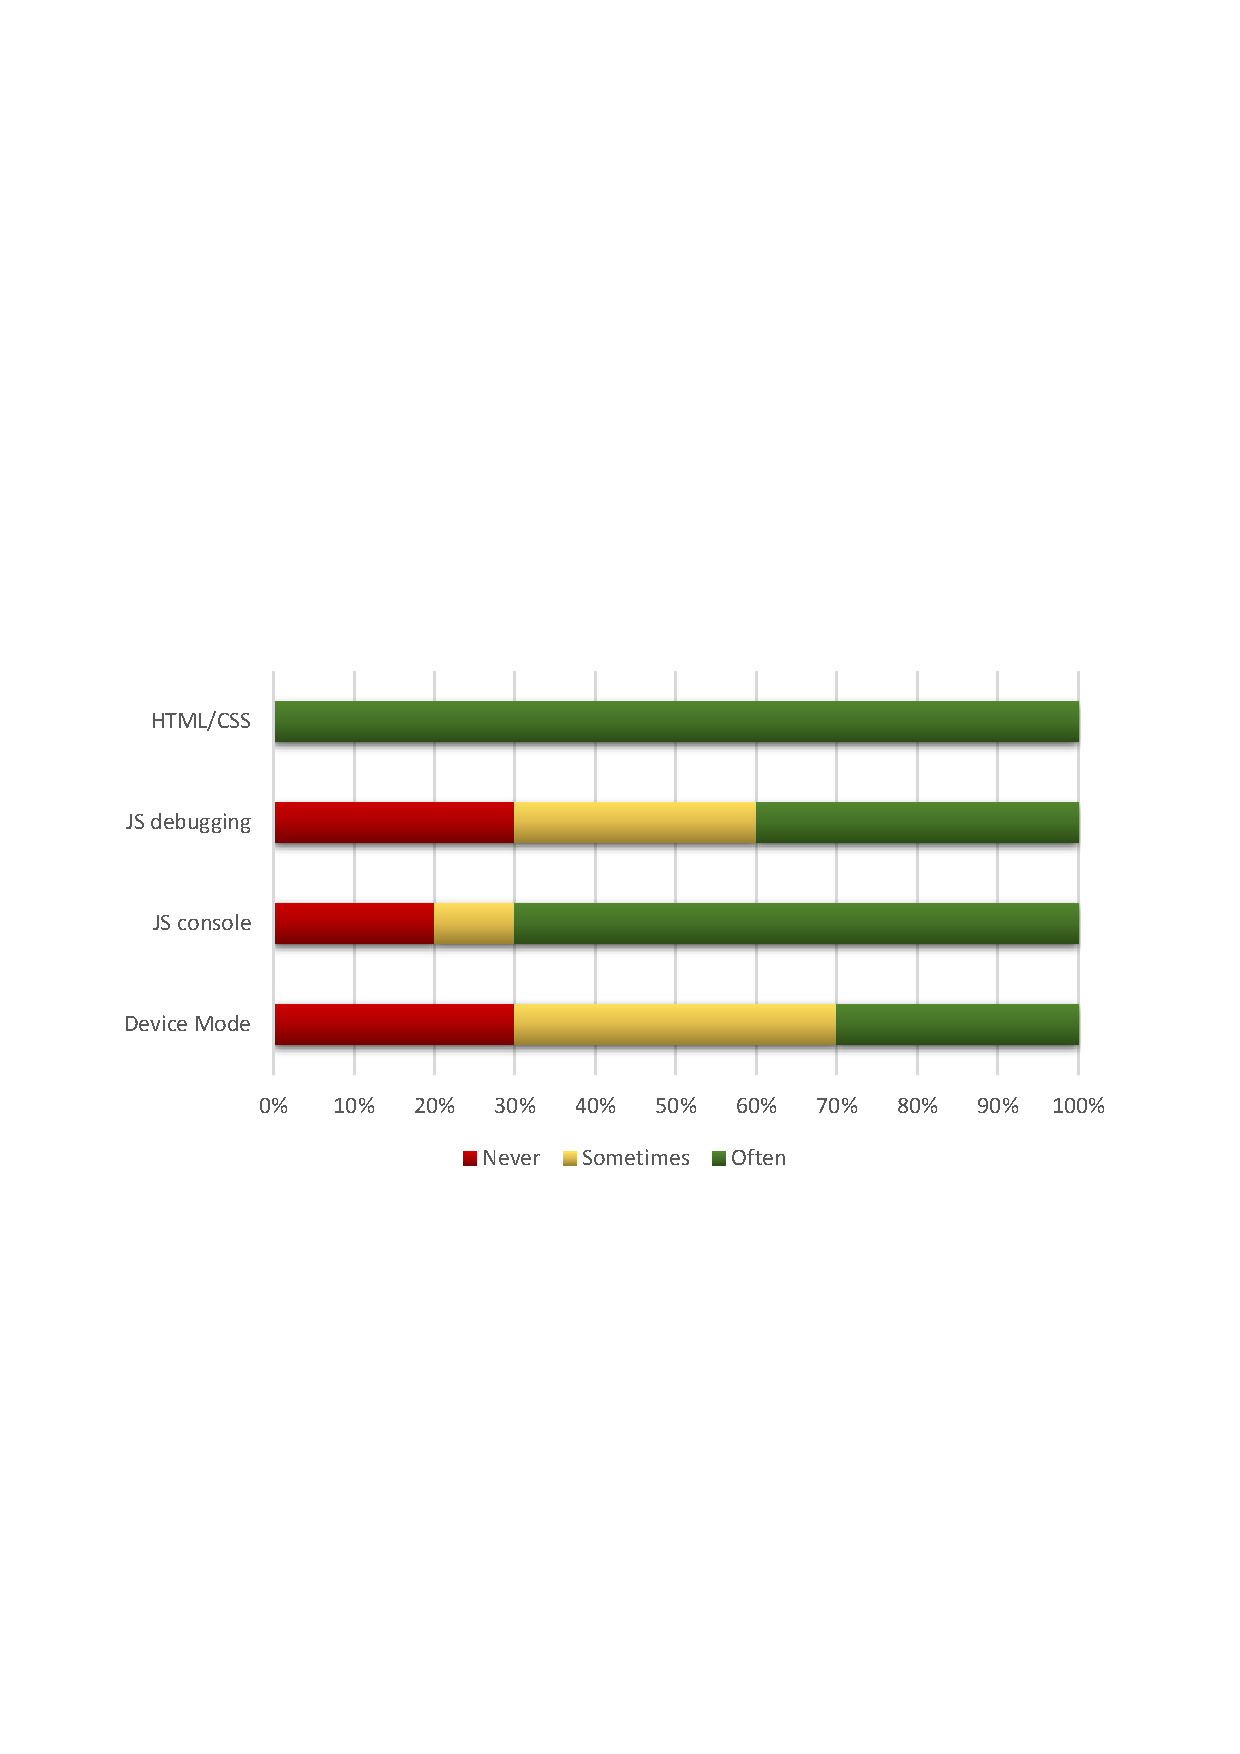
\includegraphics[width=0.8\textwidth]{images/charts/devtools_xp.pdf}
	\caption{Previous experience with Chrome DevTools}
	\label{fig:devtools_xp}
\end{figure}

\subsection{Tasks}

We used two different applications for the tasks. For each application, there were two tasks; one was about finding and fixing a bug in the code, and the other one was about implementing a new feature. The maximum time for the tasks where the participants fixed a bug was 15 minutes and the maximum time for implementing a feature was 30 minutes. After this time, we aborted the task unless it was clear that the participants would finish within the next 2 to 3 minutes. Each participant had to complete all four of the tasks; the tasks of one application with our tools, the tasks of the other application without them. The order of the applications as well as whether the first two tasks were with or without the tools was random. One of the applications was a cross-device YouTube application, called XDYouTube. The other application was a cross-device cinema application, called XDCinema.

\subsubsection{XDYouTube}
XDYouTube allows users to use their personal devices to search for videos and add them to a queue. The videos from the queue were then played one after the other on the largest of the devices. Users could also see the title and description of the currently playing video as well as the videos that are still in the queue by switching their device into landscape mode.

The first task with XDYouTube was to fix a bug concerning the video queue. As soon as one video finishes playing, the next video was dequeued from the queue and started playing. However, when no video was in the queue, a Javascript error occurred and caused the next video that was added to the queue not to play. The users were given a description of the task and then had to reproduce and fix it. 

For the second task, we asked participants to implement a remote control that could play and pause the current video. The participants had to implement two functions: One was called when the remote control button was clicked (the button as well as the event handler were already implemented), the other was called when a shared variable that states whether the video is paused or playing is changed. Thus, the participants had to change the shared variable whenever the button was clicked and to react accordingly on all devices if the shared variable changes, i.e. they had to pause or play the video on the device that plays the video and they had to change the text of the remote control button on all other devices. Furthermore, they had to change the CSS of the button such that it looked similar to a picture of a button that was given to them.

\subsubsection{XDCinema}

XDCinema allows users to search for a city and date on one device. The device then shows a list of movies that play in this city on that date as well as the cinemas where the movie is played and the time that the movie starts. If the user clicks on a cinema, a summary of the movie as well as other information about the movie is shown on another device. If the user clicks on a cinema, the location of the cinema is shown on another device.

The first task was to fix a bug where the location of most cinemas was displayed wrongly, even though the information in the database is correct. The bug was that in one function, "j" was used instead of "i", which caused a wrong location to be returned.

In the second task, the participants first had to complete the implementation of a function that shows the prices of each cinema where the movie plays below the description of the cinema. A skeleton for this function was already given where a loop over all cinemas that show the movie was already implemented, the participants only had to fill in the body of the loop. The second part was about first highlighting the correct price when the user clicks on a cinema in the search view and improving the CSS for highlighting. 

\subsection{Evaluation Methods}

\subsubsection{Questionnaires}
At the beginning of the study, each participant had to fill out a questionnaire about their background information. After every task, the participant had to fill out another questionnaire with the following questions:
\begin{itemize}
	\item It was easy to complete the task with the tools I had access to.
	\item I felt efficient completing the task with the tools I had access to.
	\item It was challenging to complete the task with the tools I had access to.
	\item The tools I had access to were well suited for completing the task.
\end{itemize}
The questions could be answered on a 5-level Likert scale from "Strongly Disagree" to "Strongly Agree". In the tasks where the participants had access to our tools, we also asked them to rate the usefulness of the individual features of the tool on a 5-level Likert scale.

After completing all tasks, the participants had to fill out a final questionnaire where they could answer some questions that compare our tools to the usual Chrome browser tools. They had to answer the following questions:
\begin{itemize}
	\item Did you find it easier to debug with or without the tool?
	\item Did you feel more efficient debugging with or without the tool?
	\item Did you prefer debugging with or without the tool?
	\item Did you find it easier to implement a feature with or without the tool?
	\item Did you feel more efficient implementing a feature with or without the tool?
	\item Did you prefer implementing a feature with or without the tool?
\end{itemize}

In addition, they also answered some general questions about our tool?
\begin{itemize}
	\item It was easy to learn how to use the tool.
	\item I felt confident using the tool.
	\item The tool was unnecessarily complex.
	\item The tool would be useful for debugging cross-device applications.
	\item The tool would be useful for implementing cross-device applications.
	\item I would use the tool for debugging cross-device applications.
	\item I would use the tool for implementing cross-device applications.
\end{itemize}
Those questions could again be answered on a 5-level Likert scale from "strongly disagree" to "strongly agree".

Finally, the participants could state which features of the tool they would use for debugging and implementing cross-device applications and they could also write some comments about the tool if they wanted to.

\subsubsection{Video Recording}
In addition to letting participants fill out questionnaires, we also used a video camera to record the participants while completing the tasks. This was mainly done to make sure that no important information was lost and so some strategies for solving tasks could be extracted from the videos. 

\subsubsection{Personal Feedback}
At the end of the study, participants were encouraged to share any comments that they still wanted to mention and to give their opinion about the tool. Any comments that the participants had given during the study were also noted.

\subsubsection{Time Measuring}
For each participant, the time required for completing each task was measured. This was mainly done to detect any major discrepancies between completion times with and without the tool. However, exact times are not considered relevant for evaluation because they highly depend on the participant and on the hints given by the instructor during the study.

\section{Results}

In the following sections, we will present the results from the individual tasks as well as the more general results. For each task, we will compare how people answered the questions in the per-task questionnaires with and without our tools. 

\subsection{XDCinema: Fixing a Bug}

The results for the task where the participants had to fix a bug in XDCinema can be seen in Figure ~\ref{fig:xdc_bug_comparison}. The figure shows the median values for the questions asked after the task with and without our tools. For the question that asks about how challenging it was to complete the task with the tools the participant had access to, a lower value is better; for all other questions, a higher value is considered better. The median values for the suitability of the tools has a rather big difference, while the differences are smaller for the other tasks. Concerning easiness and efficiency, only a very small difference in favor of our tools can be seen. One reason for the bigger difference in the suitability could be that unlike easiness and efficiency, suitability does not really depend on the task itself. In other words, if a task is difficult, the easiness will be rated lower regardless of whether our tools are used or not. On the other hand, the suitability of the tools for the task does not change with the difficulty of the task.

\begin{figure}[H]
  \centering
    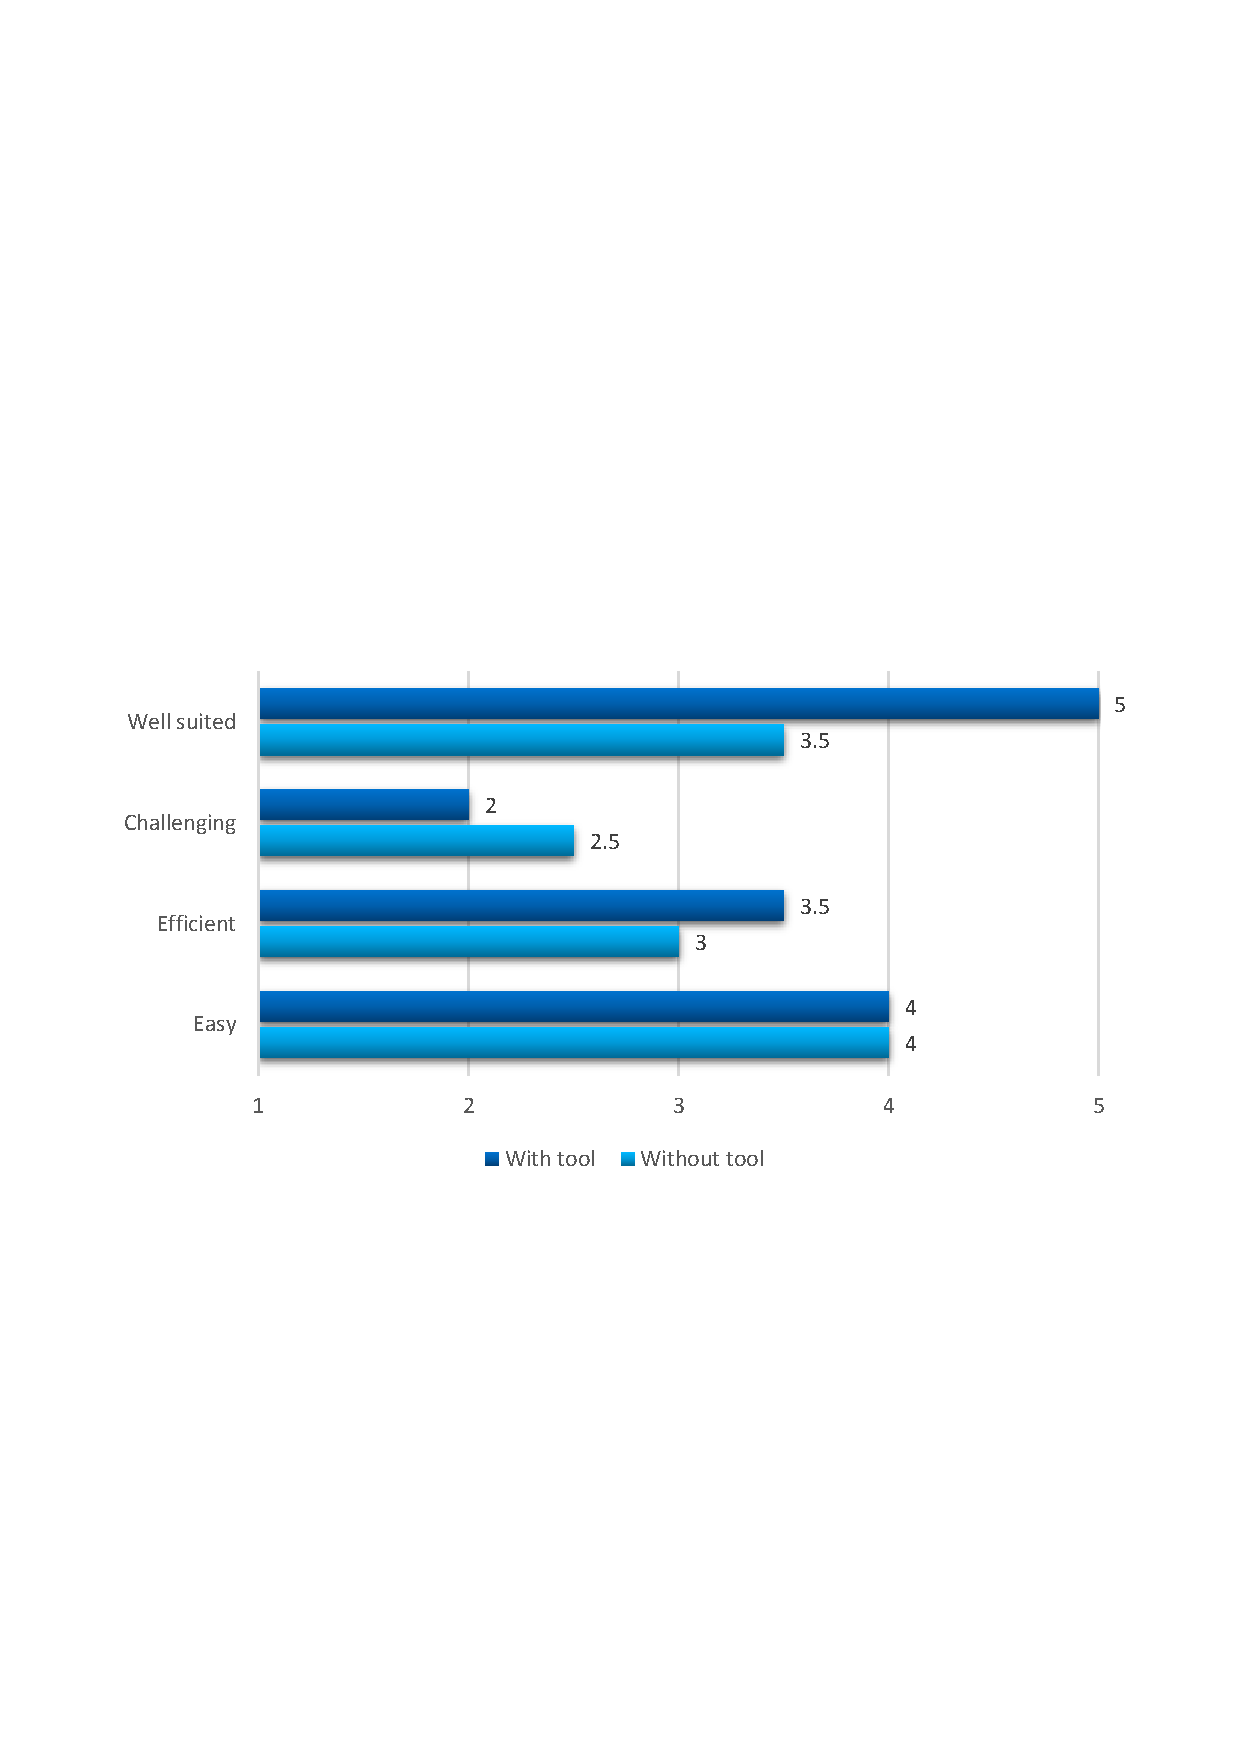
\includegraphics[width=0.8\textwidth]{images/charts/xdc_bug_comparison.pdf}
	\caption{XDCinema bug task - Comparison}
	\label{fig:xdc_bug_comparison}
\end{figure}

Figure ~\ref{fig:xdc_bug_features_used} shows how many participants used the individual features of our tools and how useful they found them. Obviously, the figure only includes the participants that had access to our tools. None of the participants used real devices and all of them used device emulation instead. However, two participants had a neutral opinion about device emulation. This could be due to the fact that the bug they had to fix is actually rather trivial and could maybe be solved faster by just looking at the code. The connection features and function debugging were used by all except one participant and were very appreciated by the participants. The shared JavaScript console was rather unpopular for this task, probably also due to the simplicity of the task and due to the fact that the bug produced no JavaScript errors that would be displayed in the console.

\begin{figure}[H]
  \centering
    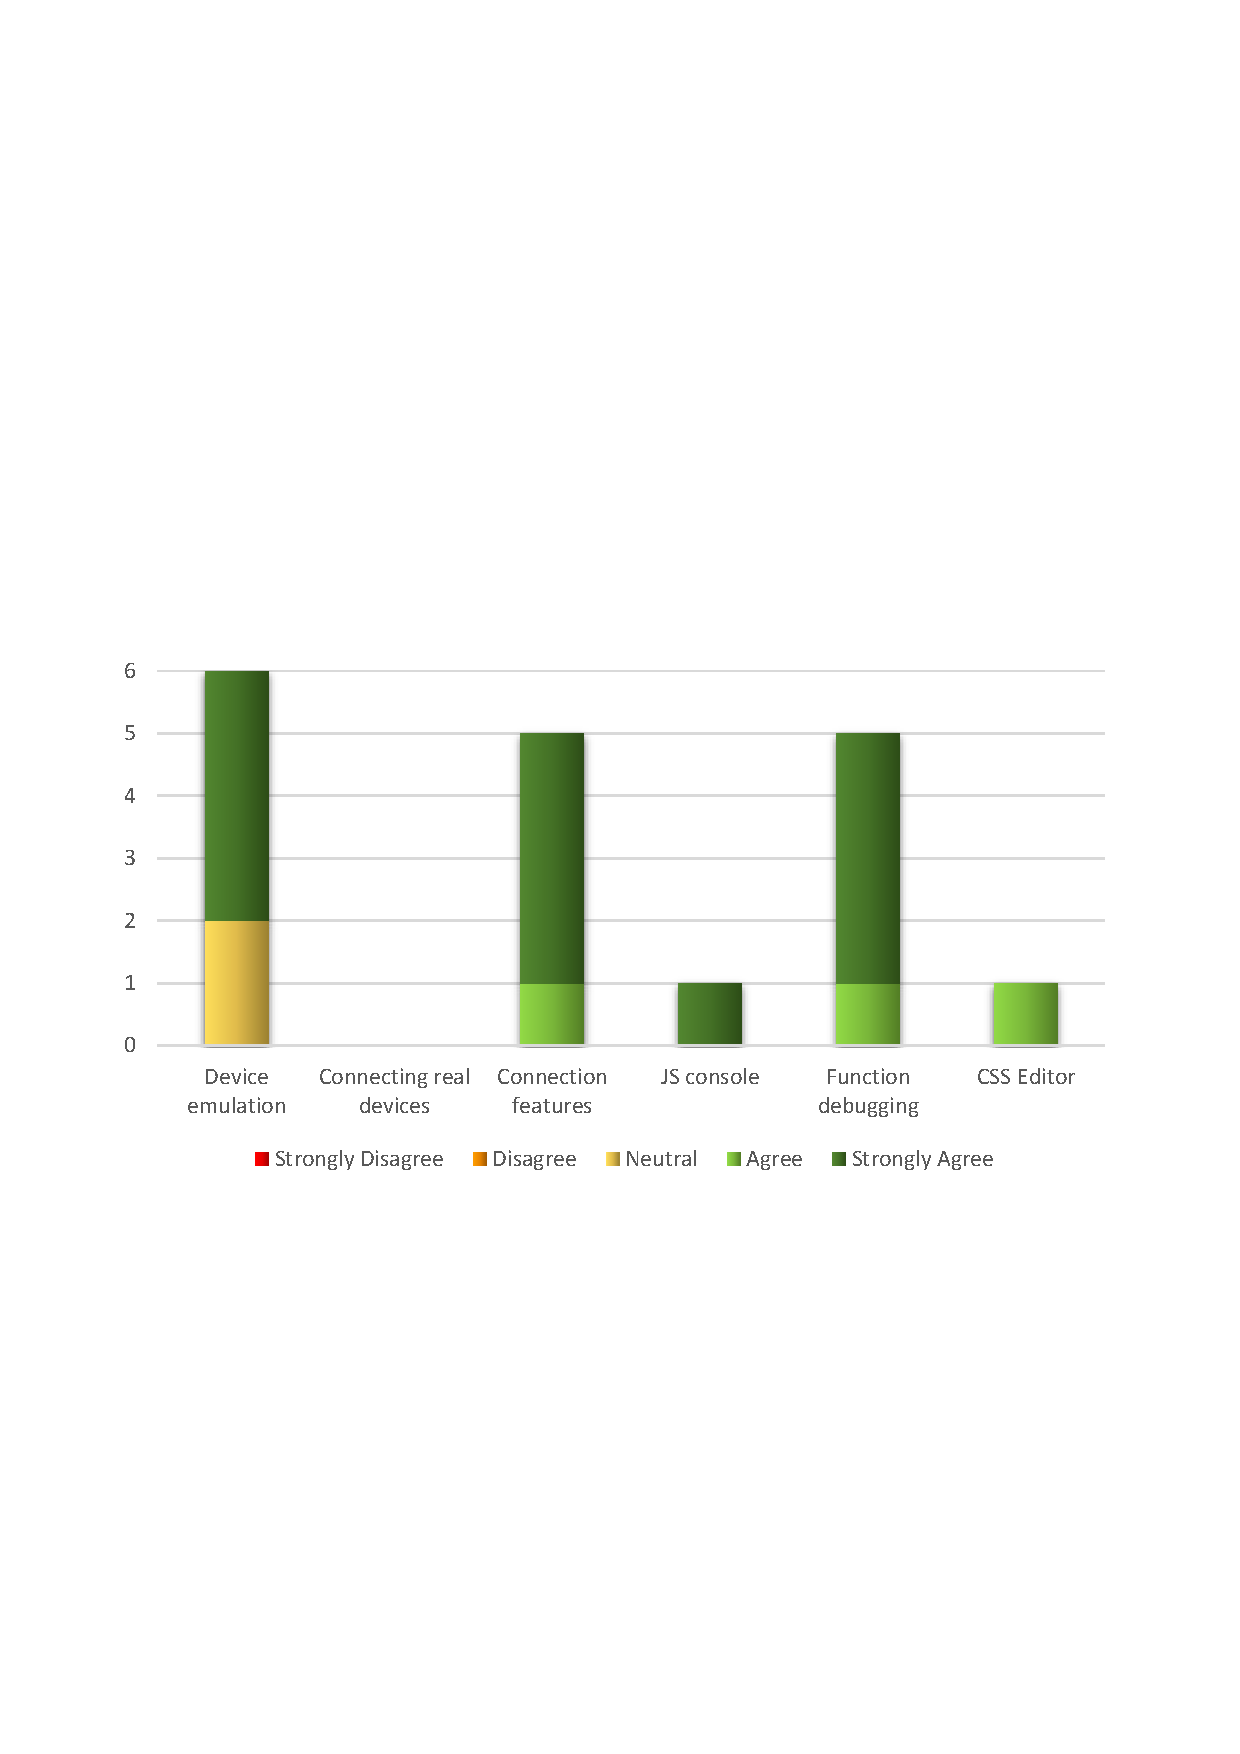
\includegraphics[width=0.8\textwidth]{images/charts/xdc_bug_features_used.pdf}
	\caption{XDCinema bug task - Features used}
	\label{fig:xdc_bug_features_used}
\end{figure}

\subsection{XDCinema: Implementing a Feature}

In Figure ~\ref{fig:xdc_impl_comparison}, the results for the implementation task in XDCinema can be seen. Again, the figure shows the median values. In this task, the difference in suitability is less pronounced than in other tasks, whereas the difference in rather large. In general, the task was considered as rather easy independent of the tools the participant had access to, although participants that had access to the tools perceived it even as a bit easier. In conclusion, it seems that the task is easy anyways, but our tools makes participants feel much more efficient when completing the task. Surprisingly, if we compare the average or median completion times for this task, the participants that had access to our tools were considerably slower. In fact, this is the only task where the difference in completion times with and without our tools is noticeable; the completion times for all other tasks are almost equivalent. However, those two facts do not necessarily contradict each other, as there were participants with very different experience levels and as it is random which participants have access to our tools and which not and the number of participants is rather low, it is possible that almost all participants with low experience fall into the same category. In general, the completion times should not be considered as especially relevant, after all the instructor also gave some hints during the study and this can also distort completion times significantly. However, it would be interesting to see how completion times differ if there is a larger number of participants. 

\begin{figure}[H]
  \centering
    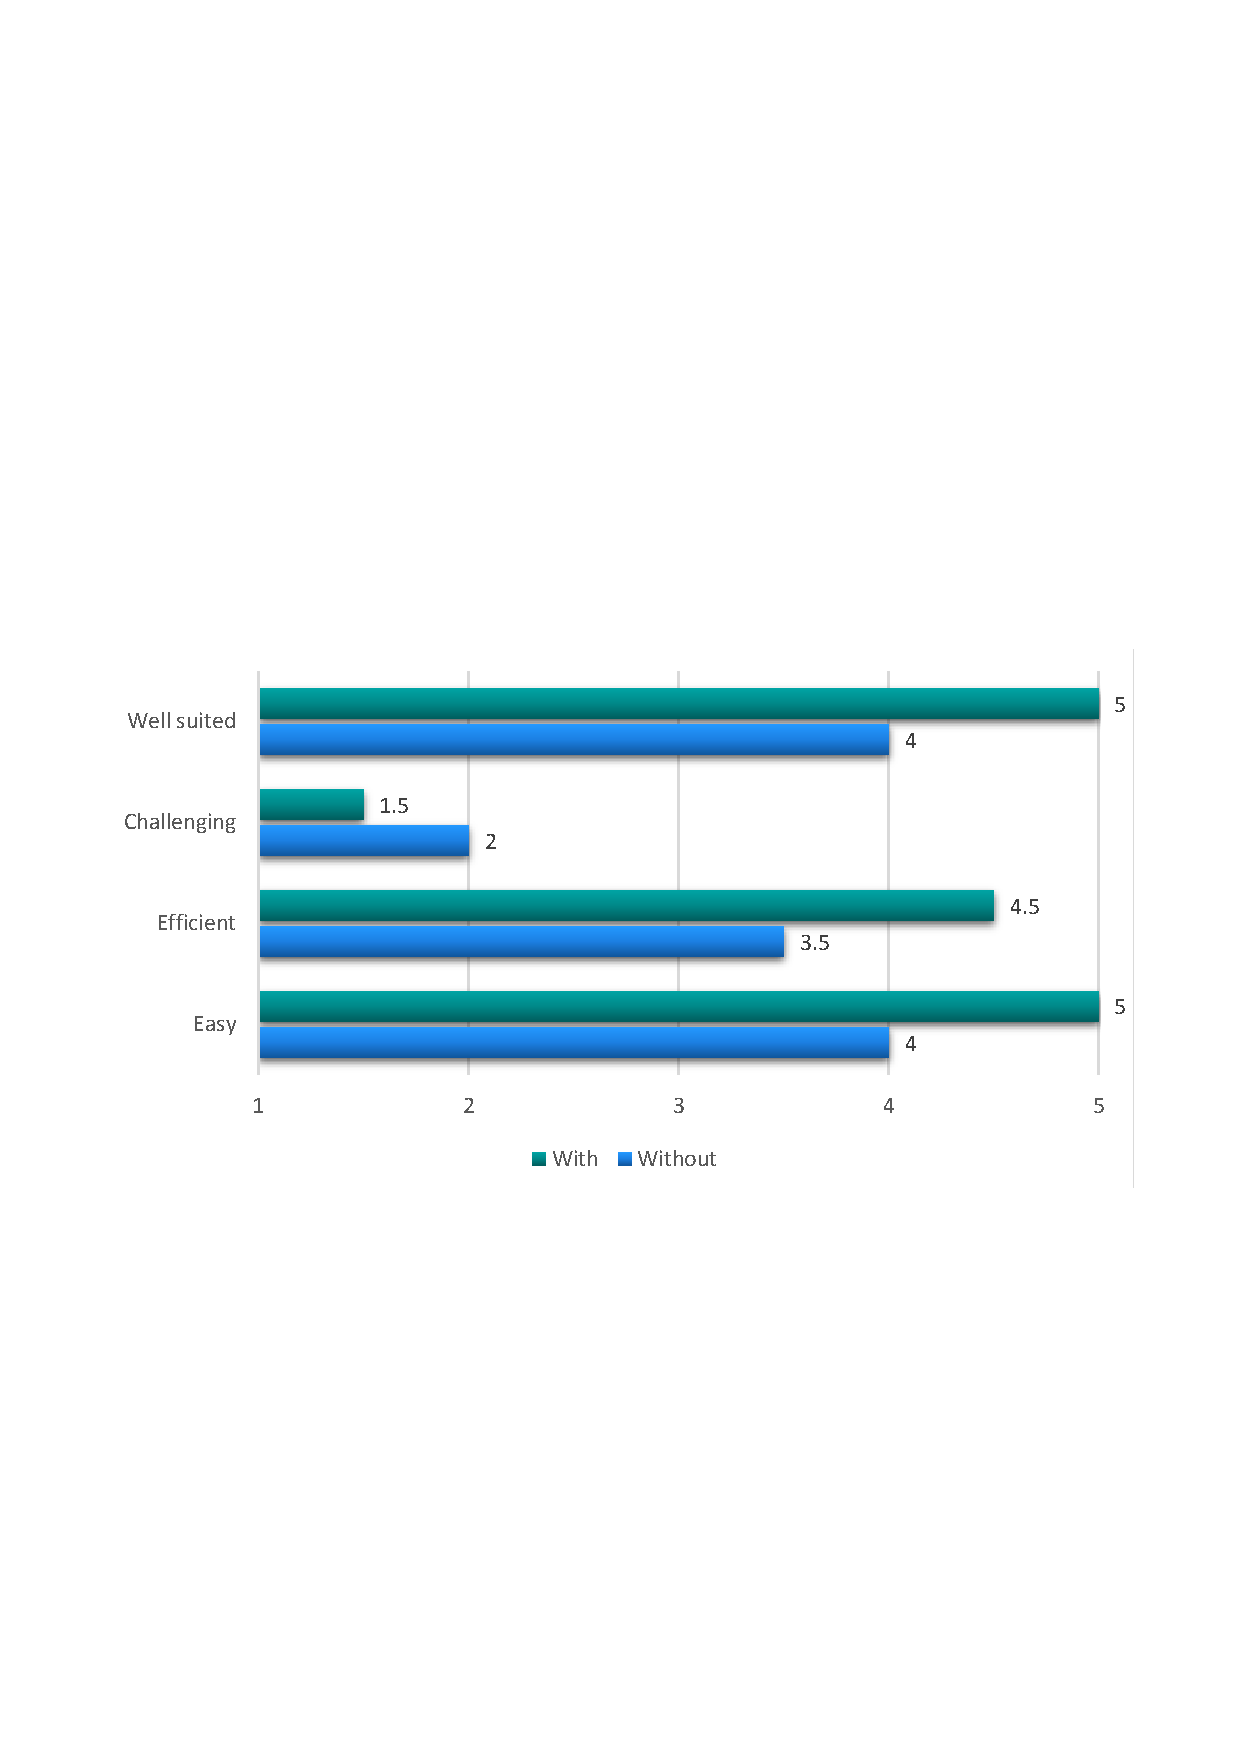
\includegraphics[width=0.8\textwidth]{images/charts/xdc_impl_comparison.pdf}
	\caption{XDCinema implementation task - Comparison}
	\label{fig:xdc_impl_comparison}
\end{figure}

Figure ~\ref{fig:xdc_impl_features_used} again shows the use and the ratings of the individual features. Again, no participant used the real devices. All participants used device emulation and the connection features and in contrast to the bug task in XDCinema, device emulation was rated as useful by all participants. Function debugging was used a bit less than in the bug task, but the shared JavaScript console was used much more. It makes sense that function debugging is used more when fixing a bug; if one implements a feature and it works immediately when testing it, there is no need to debug a function, but if one has to fix a bug, there obviously must be a bug in a function and thus it makes much more sense to debug functions. The shared JavaScript console was rarely used to send commands and most participants did not use logging for solving the task, but many participants had some syntax errors when first testing the feature and noticed the error messages in the console. This also explains why the console was used more in the implementation task than in the bug task: Generally, console outputs are very useful for debugging, but in this specific bug, there were no errors in the console in contrast to the implementation task, where syntax errors were shown in the console. Finally, the CSS editor was also used by some participants in this task. However, some completed the CSS part of the task using only the CSS file. This may be because they did not think of the CSS editor at this specific moment, or because they know CSS so well that they can just write everything down immediately. 

\begin{figure}[H]
  \centering
    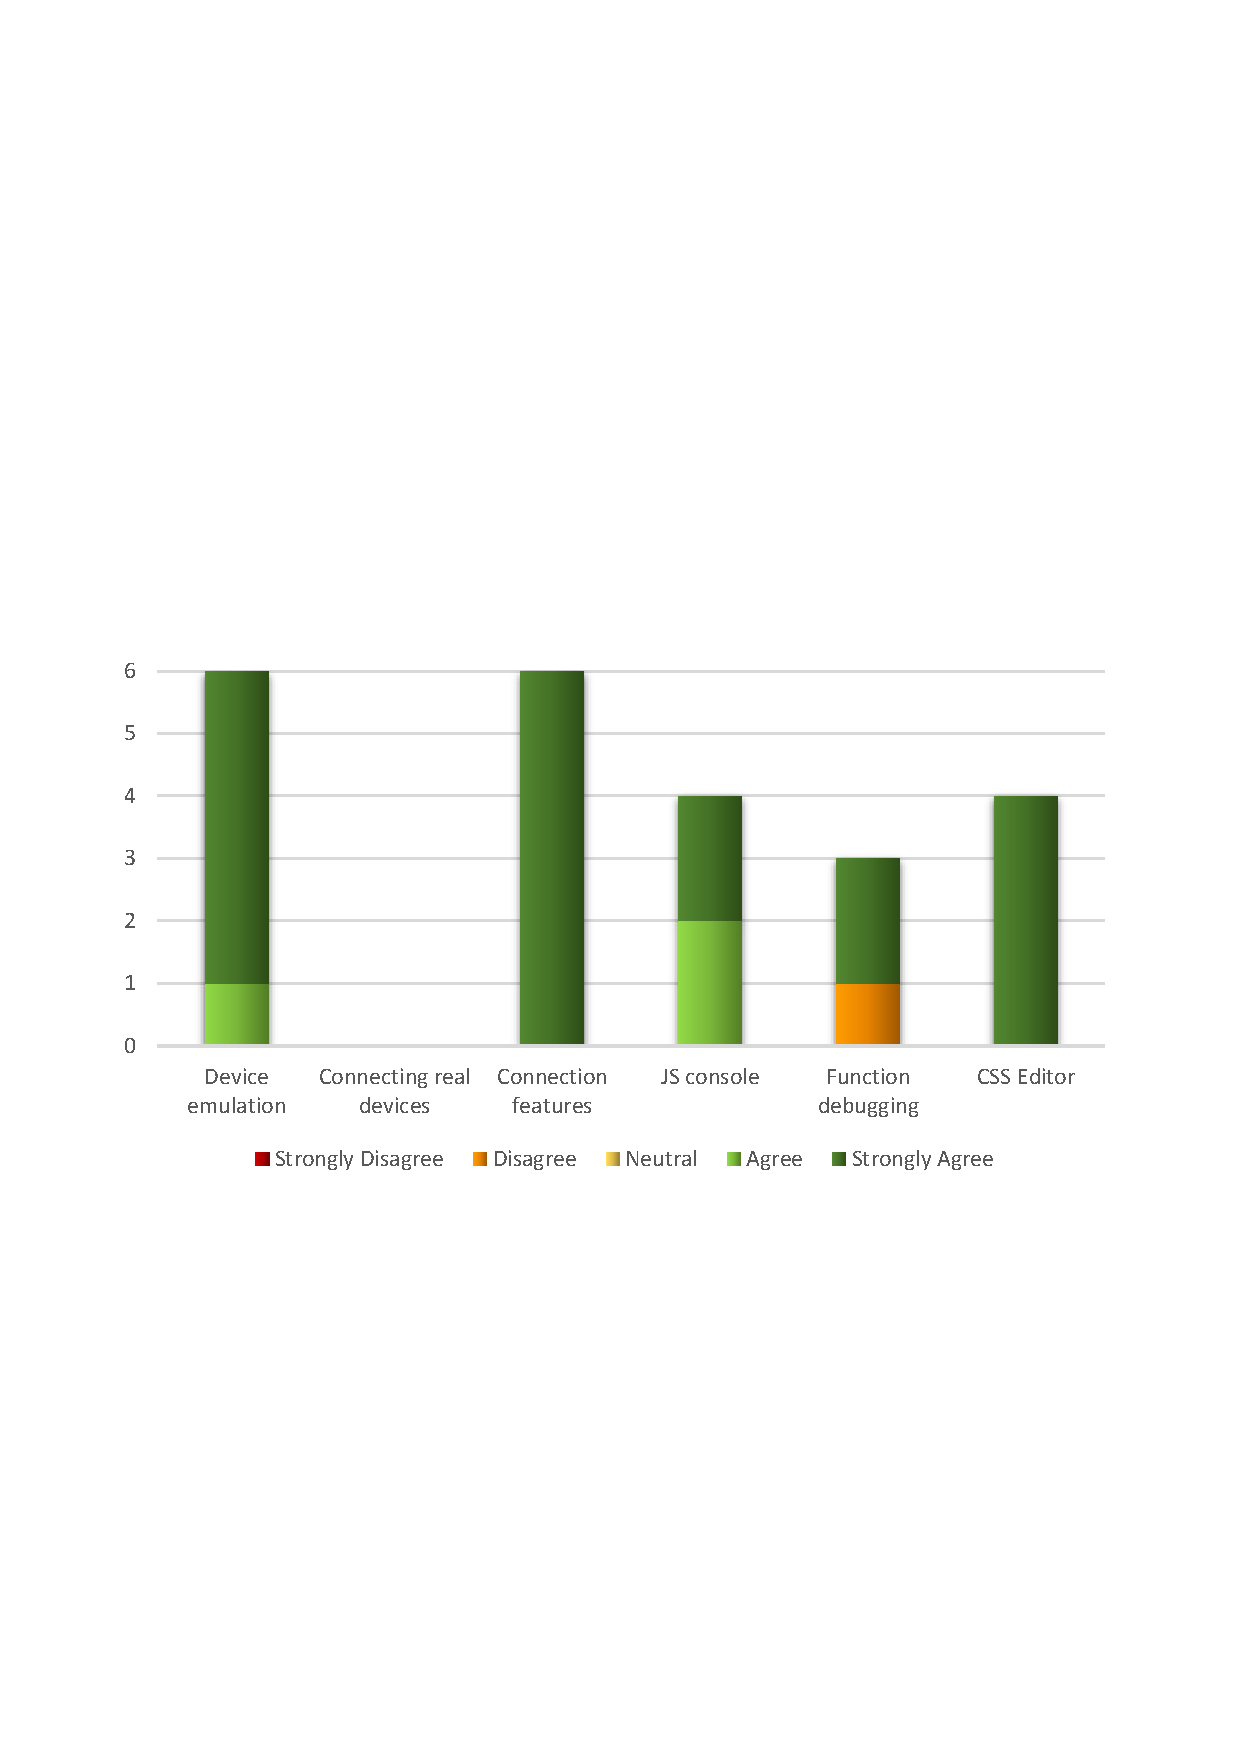
\includegraphics[width=0.8\textwidth]{images/charts/xdc_impl_features_used.pdf}
	\caption{XDCinema implementation task - Features used}
	\label{fig:xdc_impl_features_used}
\end{figure}

\subsection{XDYouTube: Fixing a Bug}

Figure ~\ref{fig:xdyt_bug_comparison} shows the results for the bug task in XDYouTube. The difference in suitability between our tools and the usual browser tools was most significant in this task with a difference of 2. The difference in efficiency is also rather large. Surprisingly, there is no difference in easiness and the task was also rated as almost equally challenging with and without our tools despite the large differences in the other questions. It seems that for this task, our tools did not make the task any easier to solve, but the participants felt more efficient when completing it. During the study, we noticed that most participants had problems reproducing the bug and almost all participants required some hints and finished the task more or less around the time limit. This could explain why the task was perceived as equally difficult with and without our tools: The participants did not really find the bug without help anyway, independent of whether they had access to our tools, so it makes sense that they would consider the task as difficult in general. 

\begin{figure}[H]
  \centering
    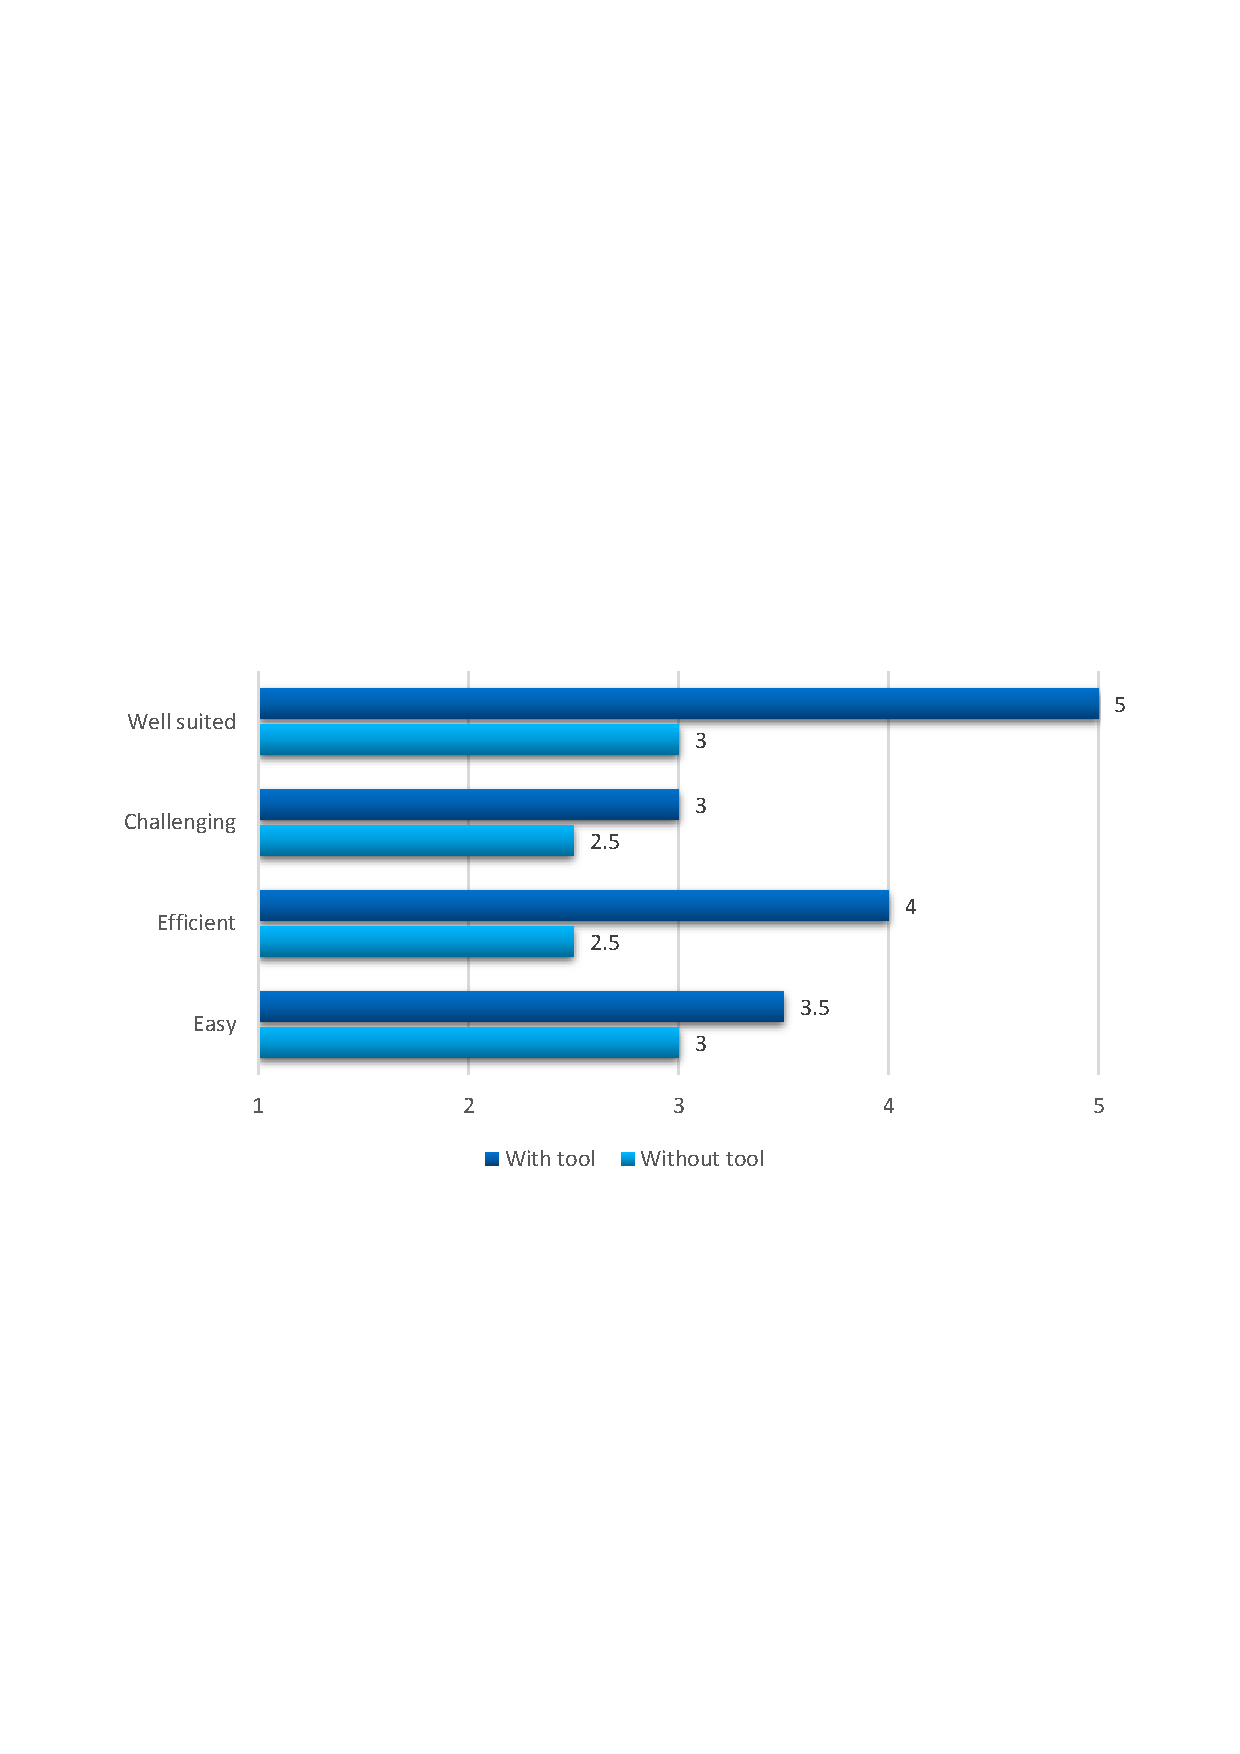
\includegraphics[width=0.8\textwidth]{images/charts/xdyt_bug_comparison.pdf}
	\caption{XDYouTube bug task - Comparison}
	\label{fig:xdyt_bug_comparison}
\end{figure}

In Figure ~\ref{fig:xdyt_bug_features_used}; the use and ratings of the individual features can be seen. All of the participants used device emulation and connection features and rated them well. Function debugging was also used by almost all participants, probably because it was difficult to reproduce the bug and the participants wanted to see what was going on in the functions. About half the participants used the shared JavaScript console, mainly to see the error produced in the function that caused the bug. One participant connected the Nexus 7 to our tools and liked the feature, but no statement about the general usefulness of the feature can be made from just one participant. 

\begin{figure}[H]
  \centering
    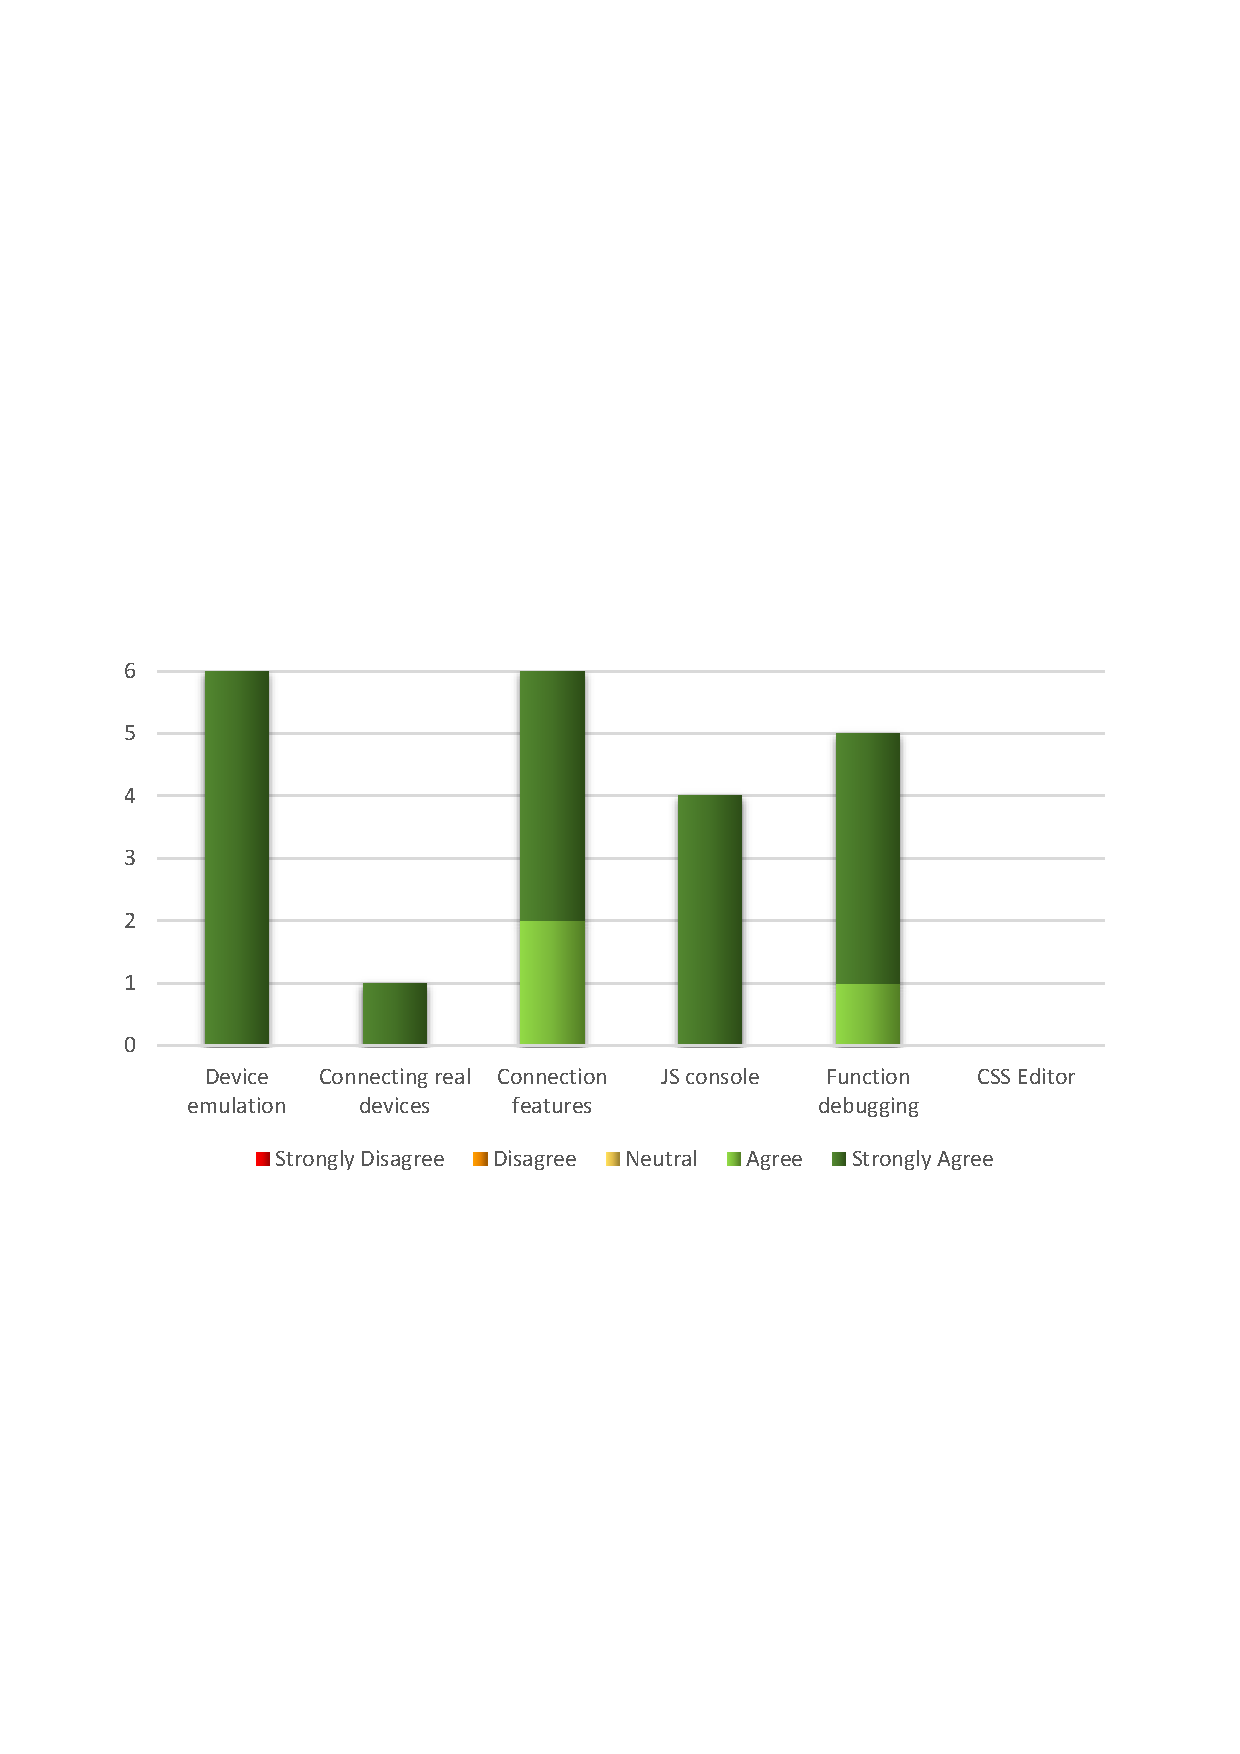
\includegraphics[width=0.8\textwidth]{images/charts/xdyt_bug_features_used.pdf}
	\caption{XDYouTube bug task - Features used}
	\label{fig:xdyt_bug_features_used}
\end{figure}

\subsection{XDYouTube: Implementing a Feature}

Figure ~\ref{fig:xdyt_impl_comparison} shows the results for the implementation task in XDYouTube. In this task, all questions were clearly rated in favor of our tools. While the participant answered the questions in a rather neutral way when they did not have access to our tools, they clearly stated that the task was easy to complete and felt efficient to complete with our tools. This task differs from the others a bit, because all other tasks had questions where the difference in median was 0.5 or 0, whereas the difference is at least 1 in this task for every question.

\begin{figure}[H]
  \centering
    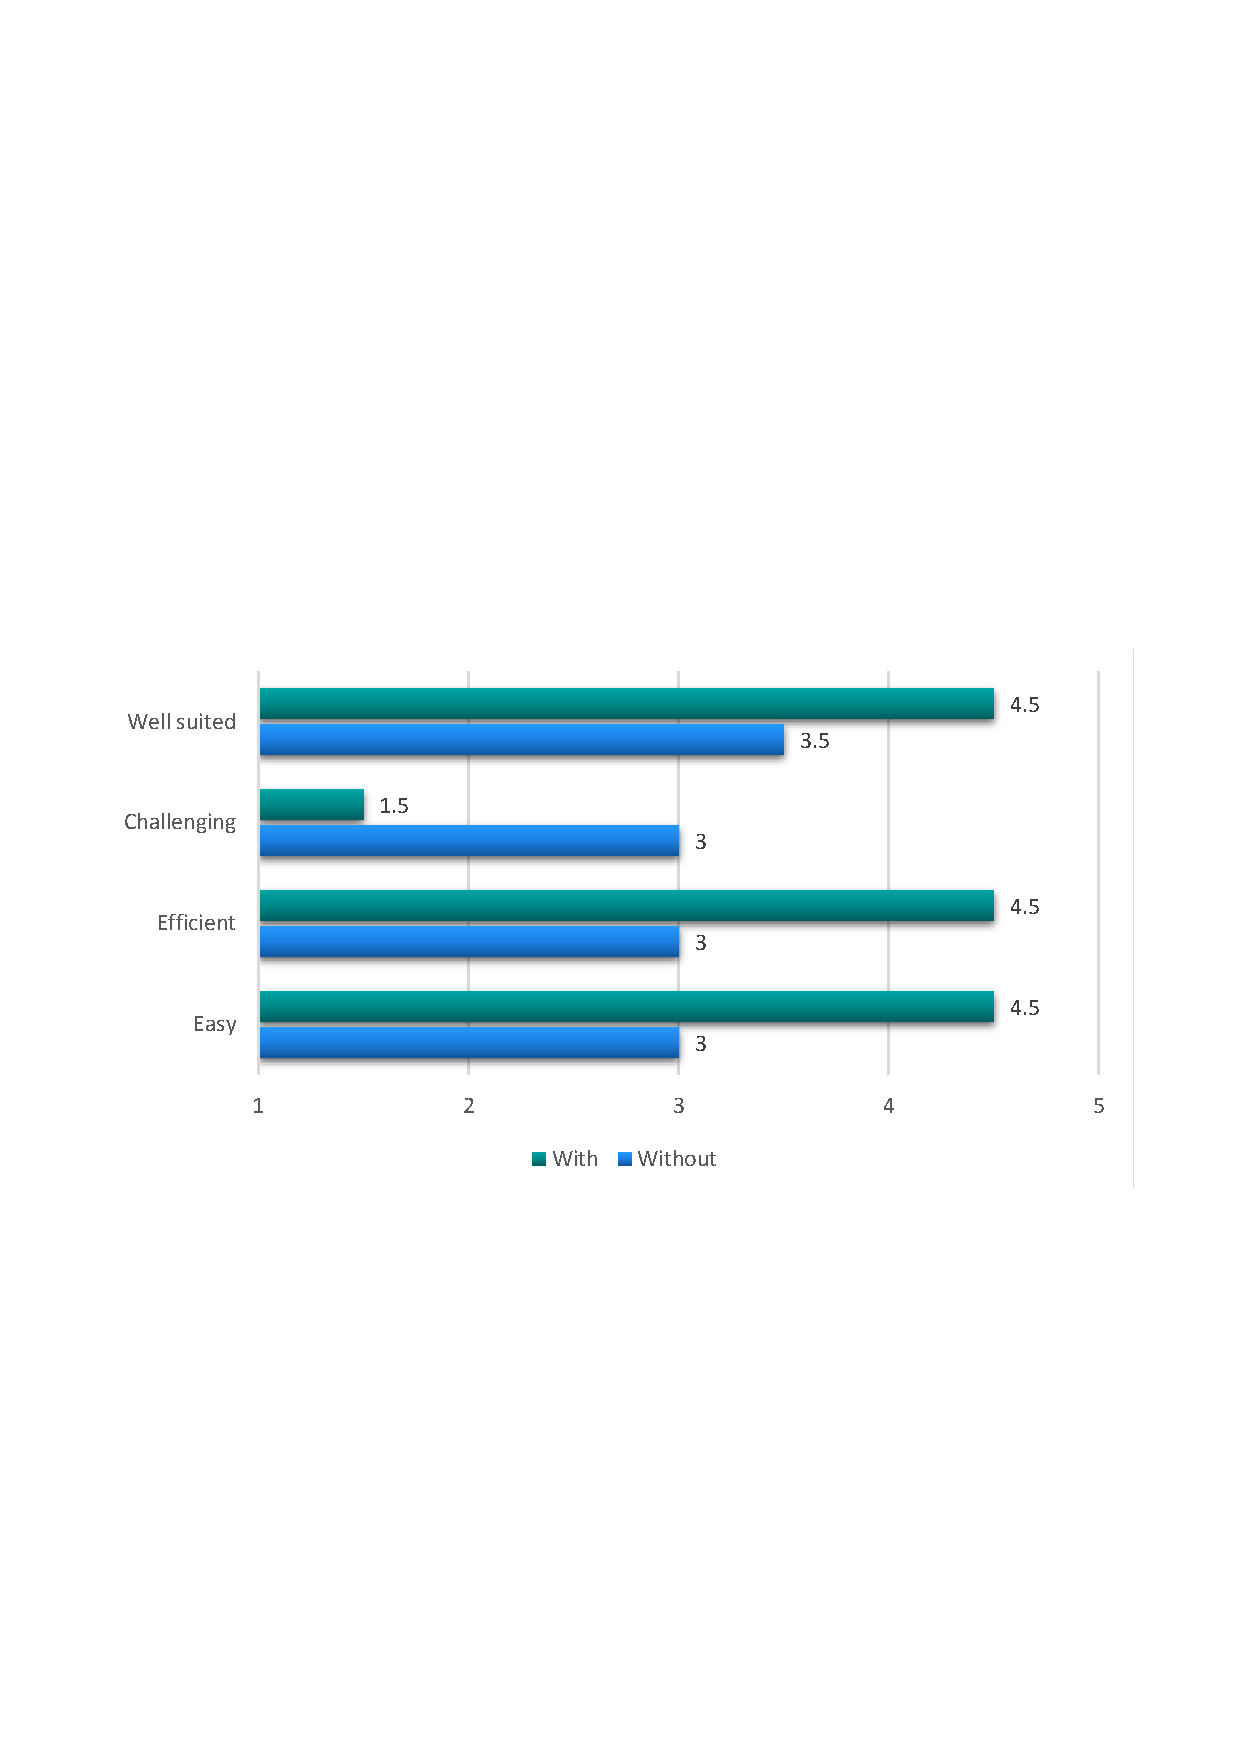
\includegraphics[width=0.8\textwidth]{images/charts/xdyt_impl_comparison.pdf}
	\caption{XDYouTube implementing task - Comparison}
	\label{fig:xdyt_impl_comparison}
\end{figure}

In Figure ~\ref{fig:xdyt_impl_features_used}; the use and ratings of the individual features can be seen. Once again, device emulation and the connection features were used by every participant. The shared JavaScript console and CSS editor were about equally popular and rated as very useful except for one participant that had a neutral opinion on the console. Function debugging was rarely used for this task. This is rather surprising because many participants had a bug where they had switched playing and pausing the video at the beginning and this could probably have been solved easily by debugging the function. However, most participants just got stuck at the bug and required some hints to fix it instead of debugging their functions. Those participants were in the same group as the one that required significantly longer for solving the implementation task in XDCinema which could again indicate that the participants in this group had a bit lower experience in web application development. When comparing the web application development experience stated in the general questionnaire by the two groups, the other group has a median experience of 4.5 while this one has a median experience of 3.5, so there indeed seems to be some difference in experience levels.

\begin{figure}[H]
  \centering
    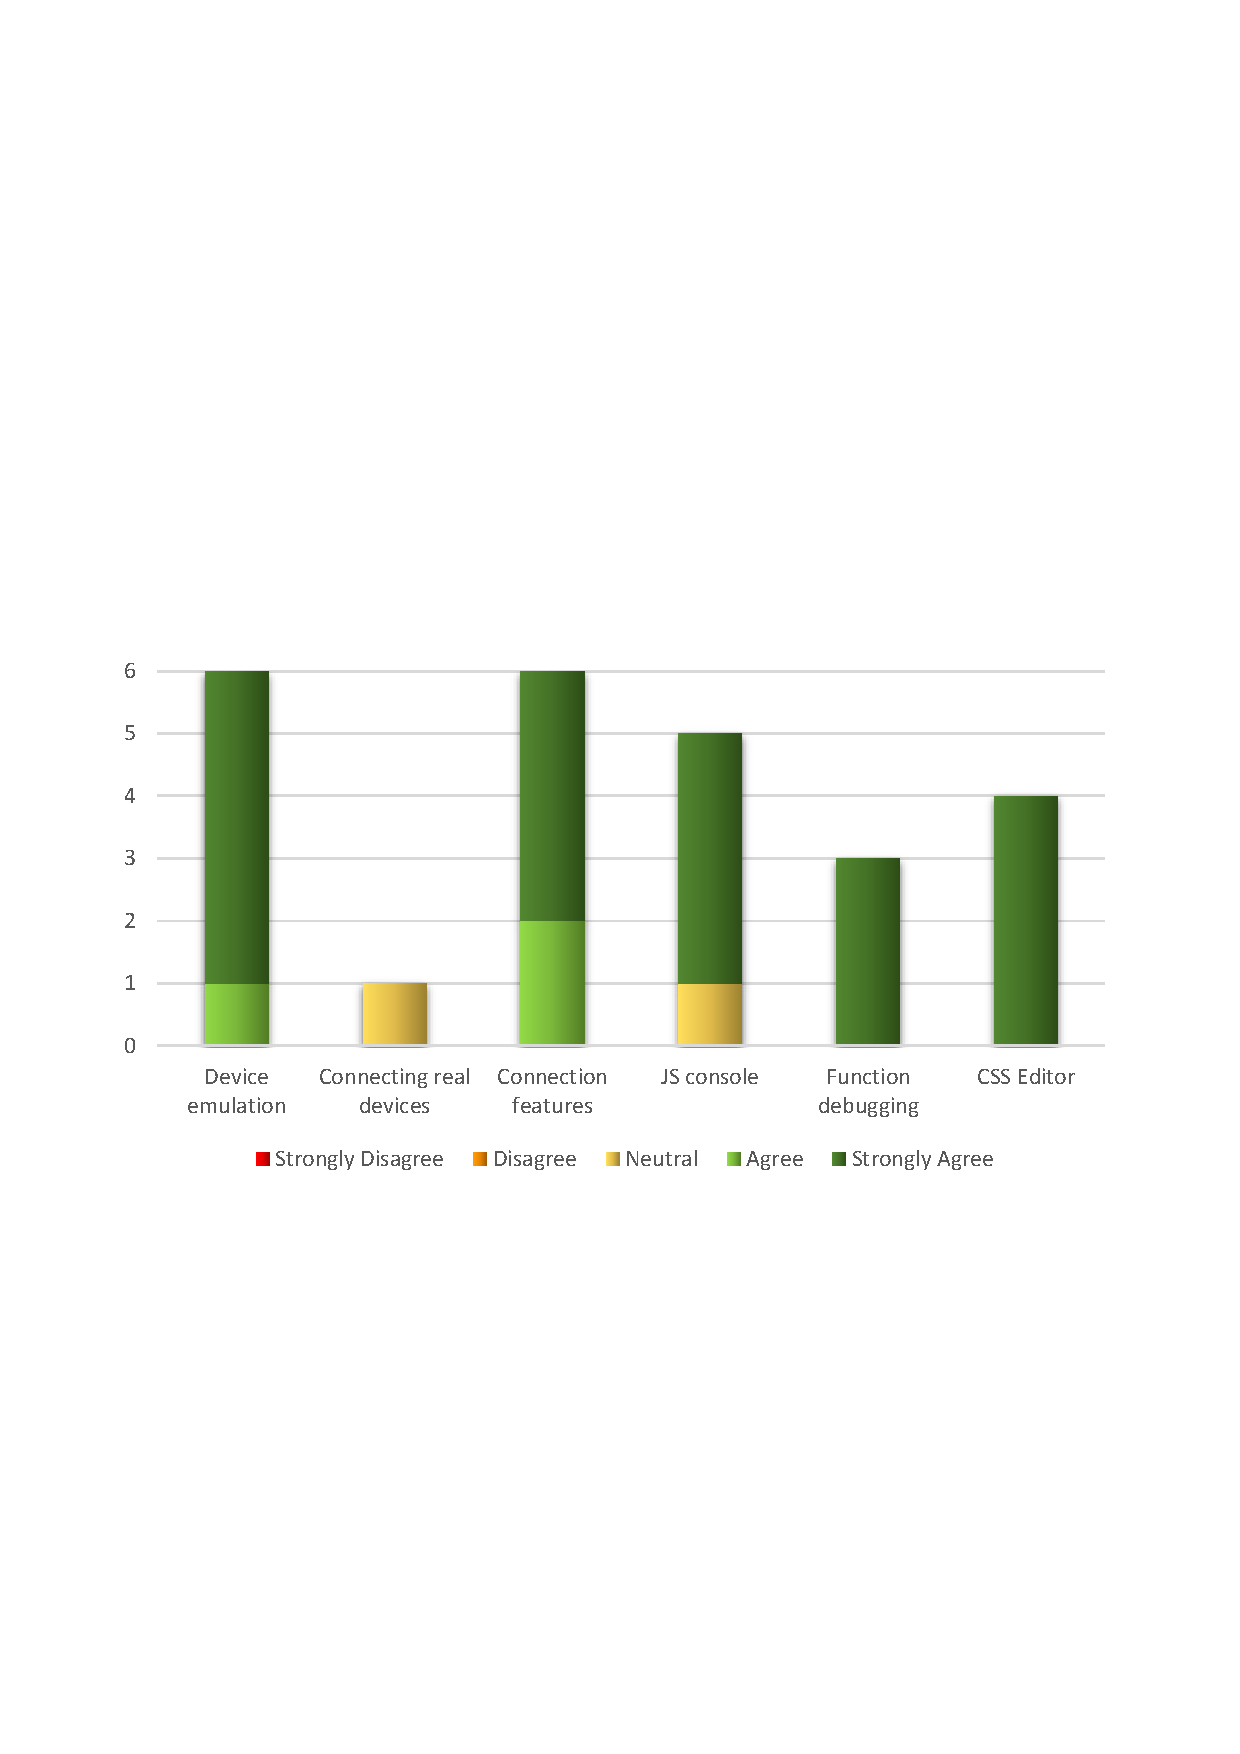
\includegraphics[width=0.8\textwidth]{images/charts/xdyt_impl_features_used.pdf}
	\caption{XDYouTube implementing task - Features used}
	\label{fig:xdyt_impl_features_used}
\end{figure}

\subsection{General}

In general, our tools were rated as very useful for all tasks with a median value of 5 for every task. In contrast, the usefulness of the usual browser tools was rated with median values between 3 and 4, thus we consider our tools as useful for implementing and debugging cross-device applications. The efficiency was also rated as significantly better for all tasks except the bug task in XDCinema, where the difference was only 0.5. This indicates that our tools make the process of testing cross-device applications more efficient. The difference in easiness seems to depend partially on the type of task; in the tasks where the participants had to implement a feature, completing the task with out tools was clearly considered easier, whereas the difference was smaller for the tasks where the participants had to fix a bug. Surprisingly, the results for the question about how challenging it was to complete the task do not necessarily relate to the results of the question about easiness. For the bug task in XDCinema and the implementation task in XDYouTube, our tools seem to make the task less challenging, but for the other two tasks, the differences are very minor. In the XDYouTube bug task, completing the task with our tools is even rated as slightly more challenging.

\section{Discussion}

Figure ~\ref{fig:implementing_easier} shows that about three quarters of all participants considered implementing a feature easier with our tools. Only one participant found it easier to implement a feature without our tools. However, in principle, this option is redundant as the participants still have access to the browser tools even when they have access to our tools. Thus the relevant conclusion is that about one quarter of the participants did not see any gain in easiness from using our tools. The same applies to the question about whether implementing a feature feels more efficient with our tools (see Figure ~\ref{fig:implementing_efficient}); this figure shows exactly the same results as the figure about easiness. However, all except one participant preferred implementing a feature with our tools (see Figure ~\ref{fig:prefer_implementing}). Thus, it seems that participants like to have access to our tools even if they cannot directly relate them to a decrease in difficulty or to an increase in efficiency.

\begin{figure}[H]
  \centering
    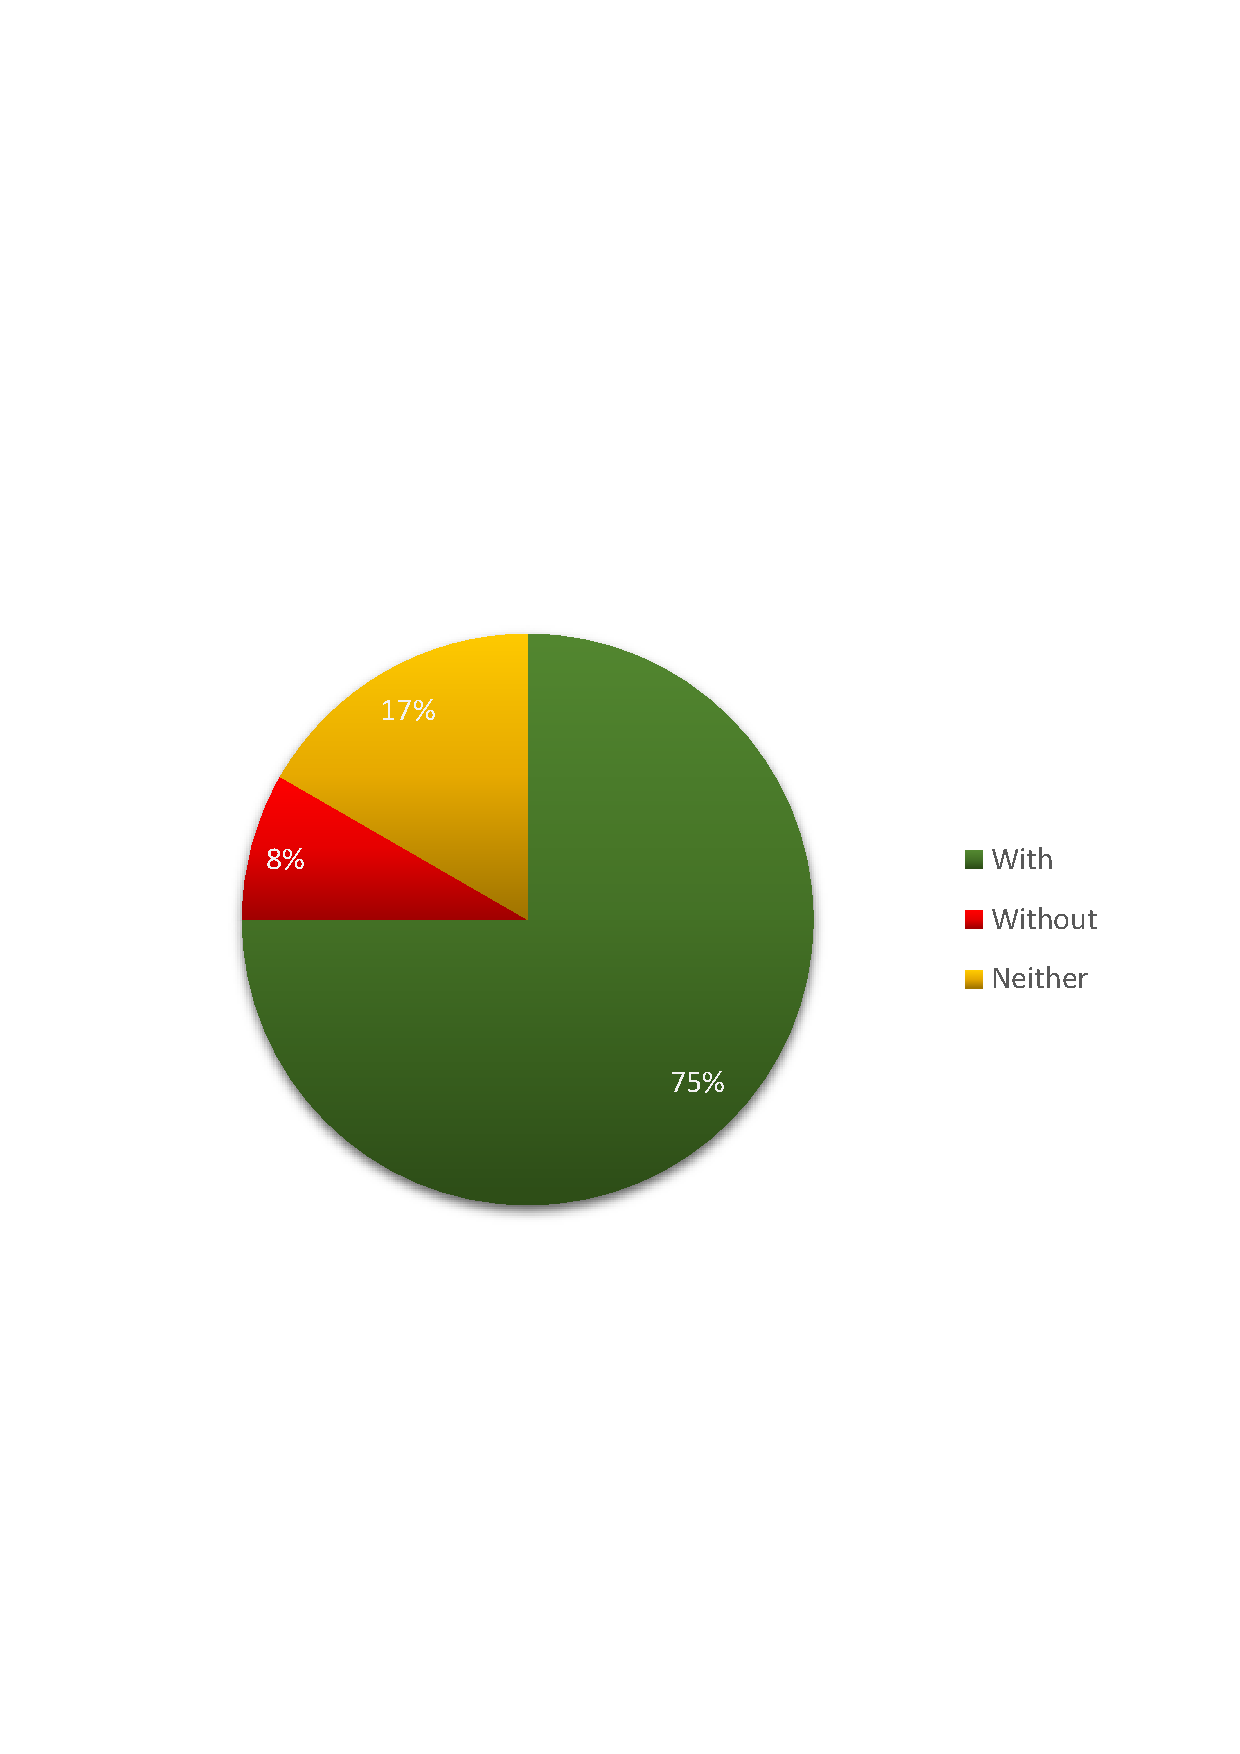
\includegraphics[width=0.6\textwidth]{images/charts/implementing_easier.pdf}
	\caption{Easiness of implementing a feature}
	\label{fig:implementing_easier}
\end{figure}

\begin{figure}[H]
  \centering
    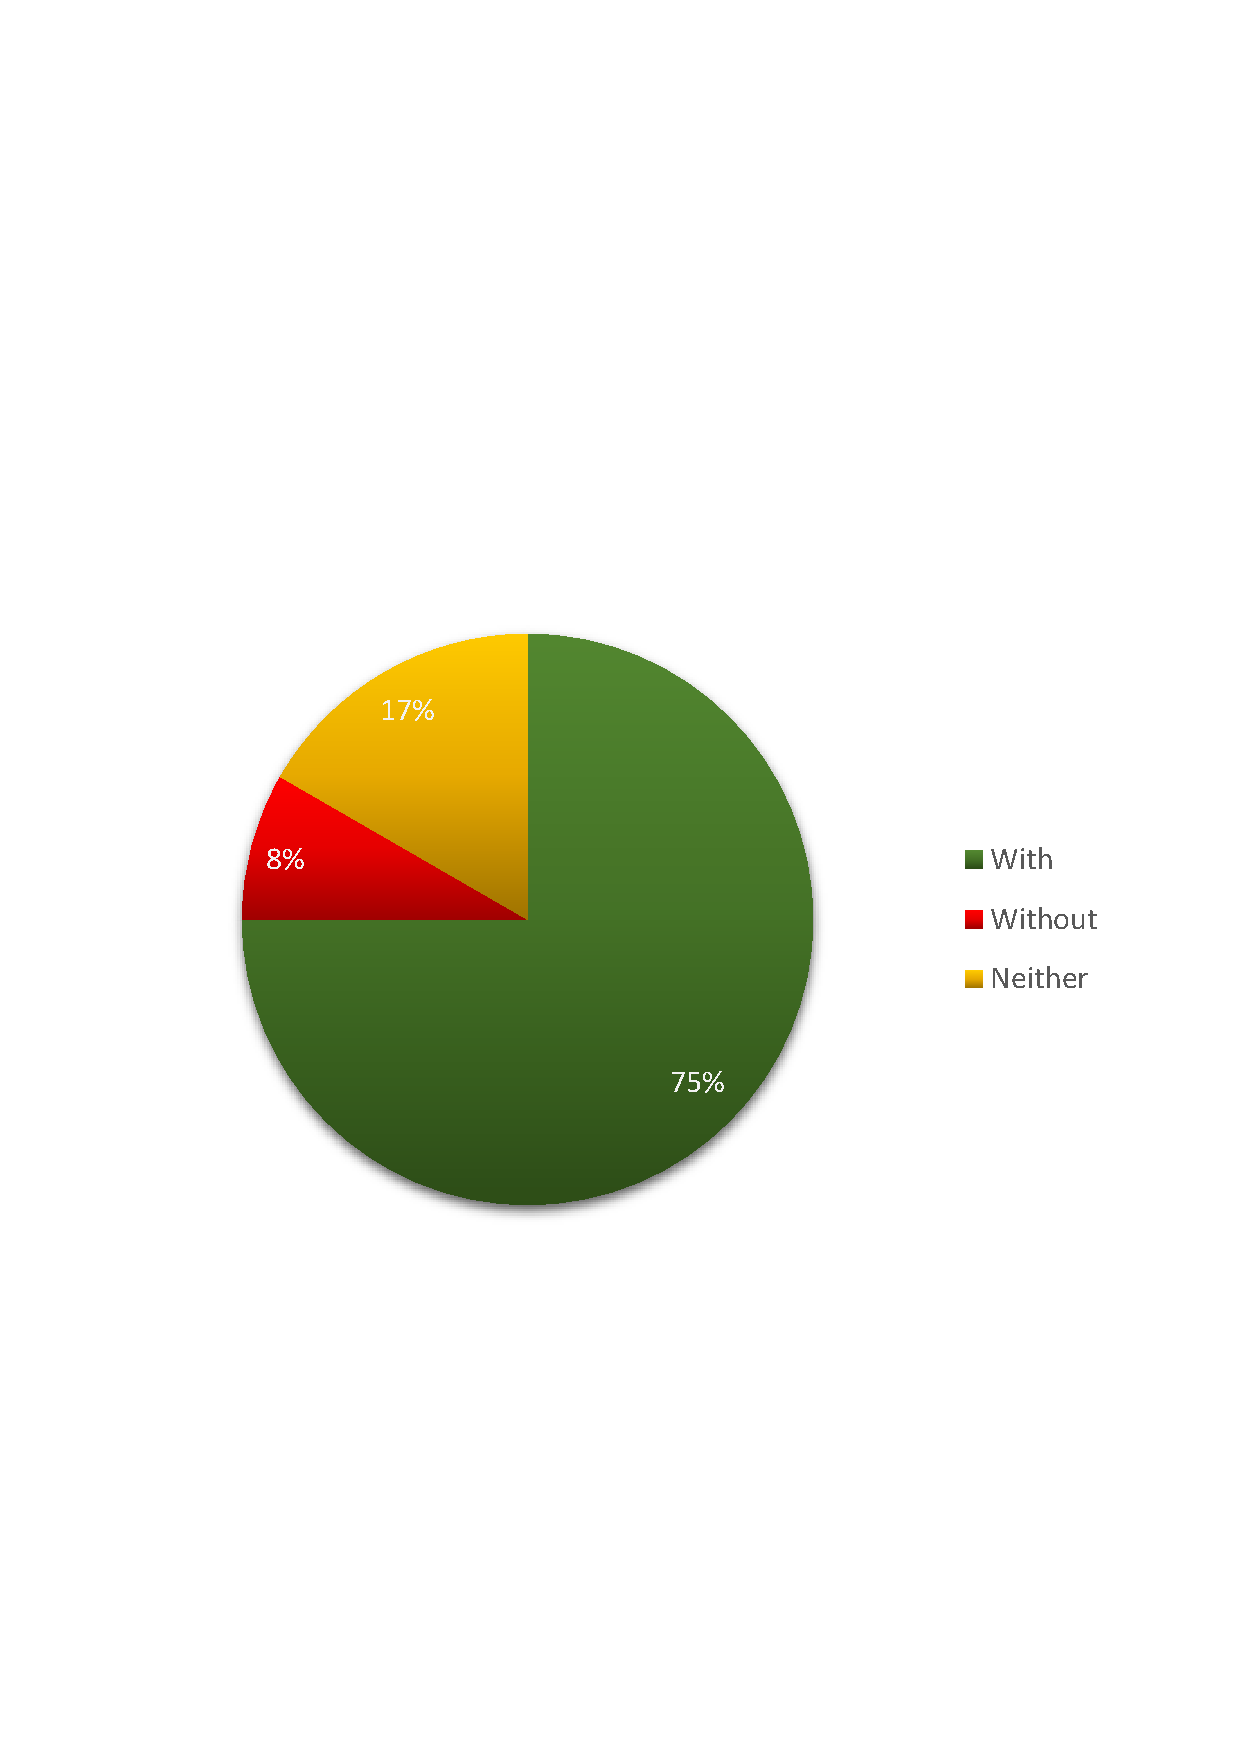
\includegraphics[width=0.6\textwidth]{images/charts/implementing_efficient.pdf}
	\caption{Efficiency of implementing a feature}
	\label{fig:implementing_efficient}
\end{figure}

\begin{figure}[H]
  \centering
    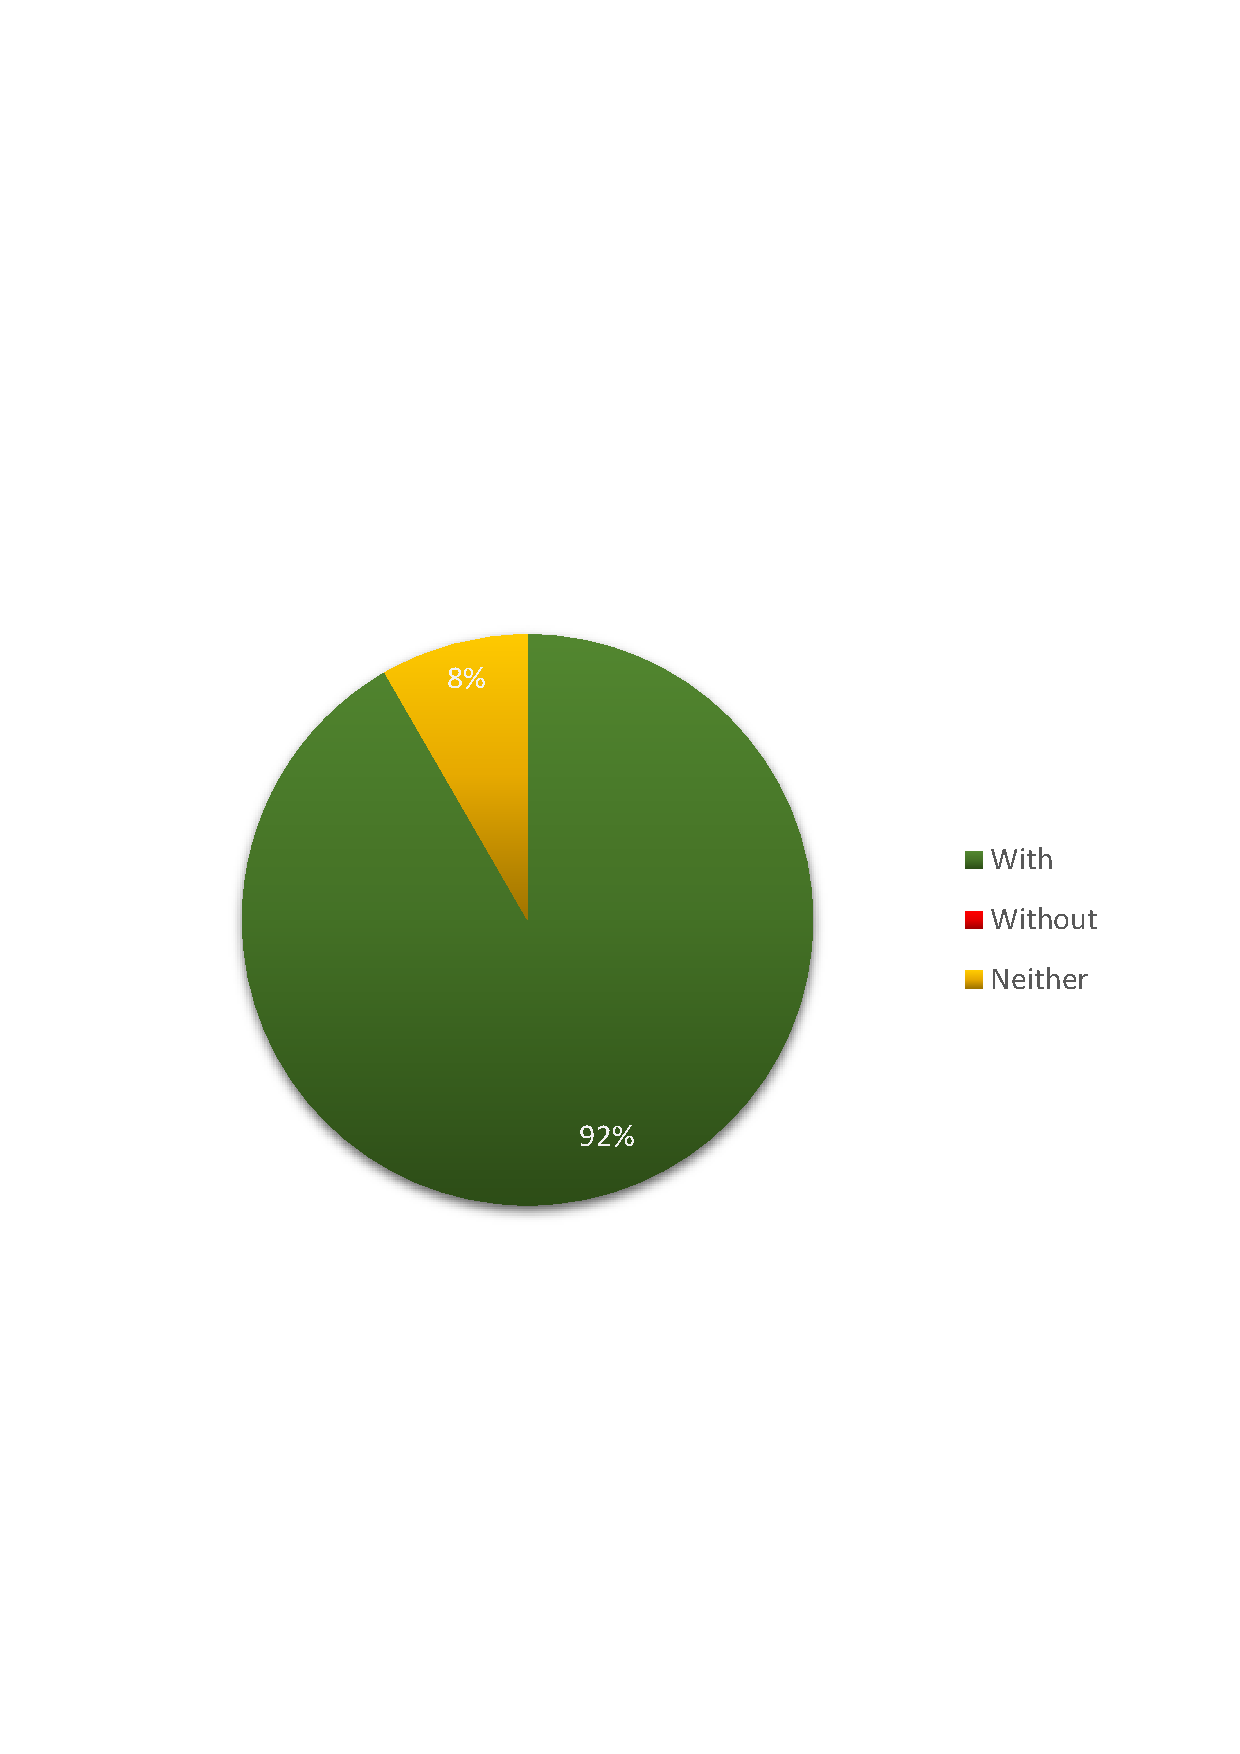
\includegraphics[width=0.6\textwidth]{images/charts/prefer_implementing.pdf}
	\caption{Preference for implementing a feature}
	\label{fig:prefer_implementing}
\end{figure}

Figure ~\ref{fig:debugging_easier} shows that most participants found it easier to debug a cross-device application with our tools. The results get even more clear if we look at Figure ~\ref{fig:debugging_efficient} and Figure ~\ref{prefer_debugging}. Those two figures show that all participants felt more efficient when debugging with our tools and also preferred debugging with our tools.

\begin{figure}[H]
  \centering
    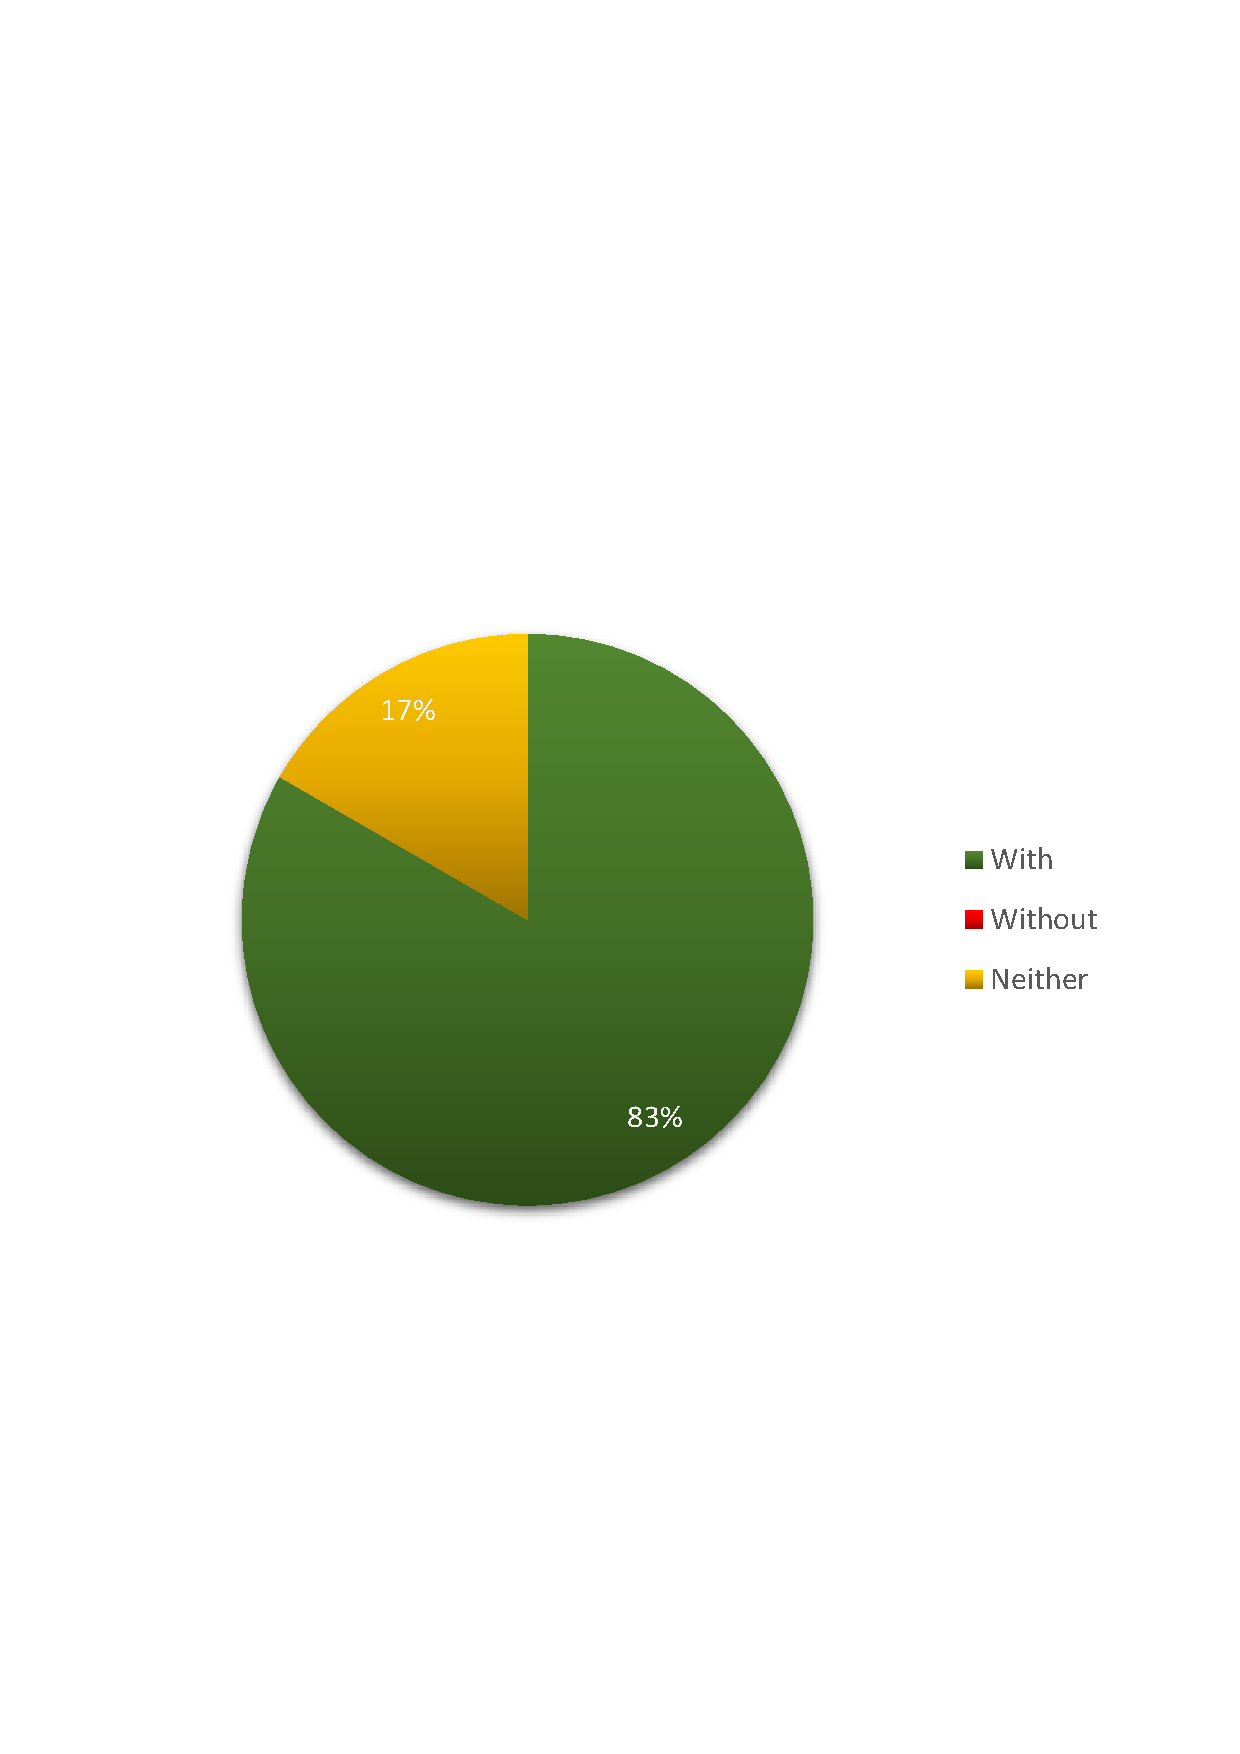
\includegraphics[width=0.6\textwidth]{images/charts/debugging_easier.pdf}
	\caption{Easiness of debugging}
	\label{fig:debugging_easier}
\end{figure}

\begin{figure}[H]
  \centering
    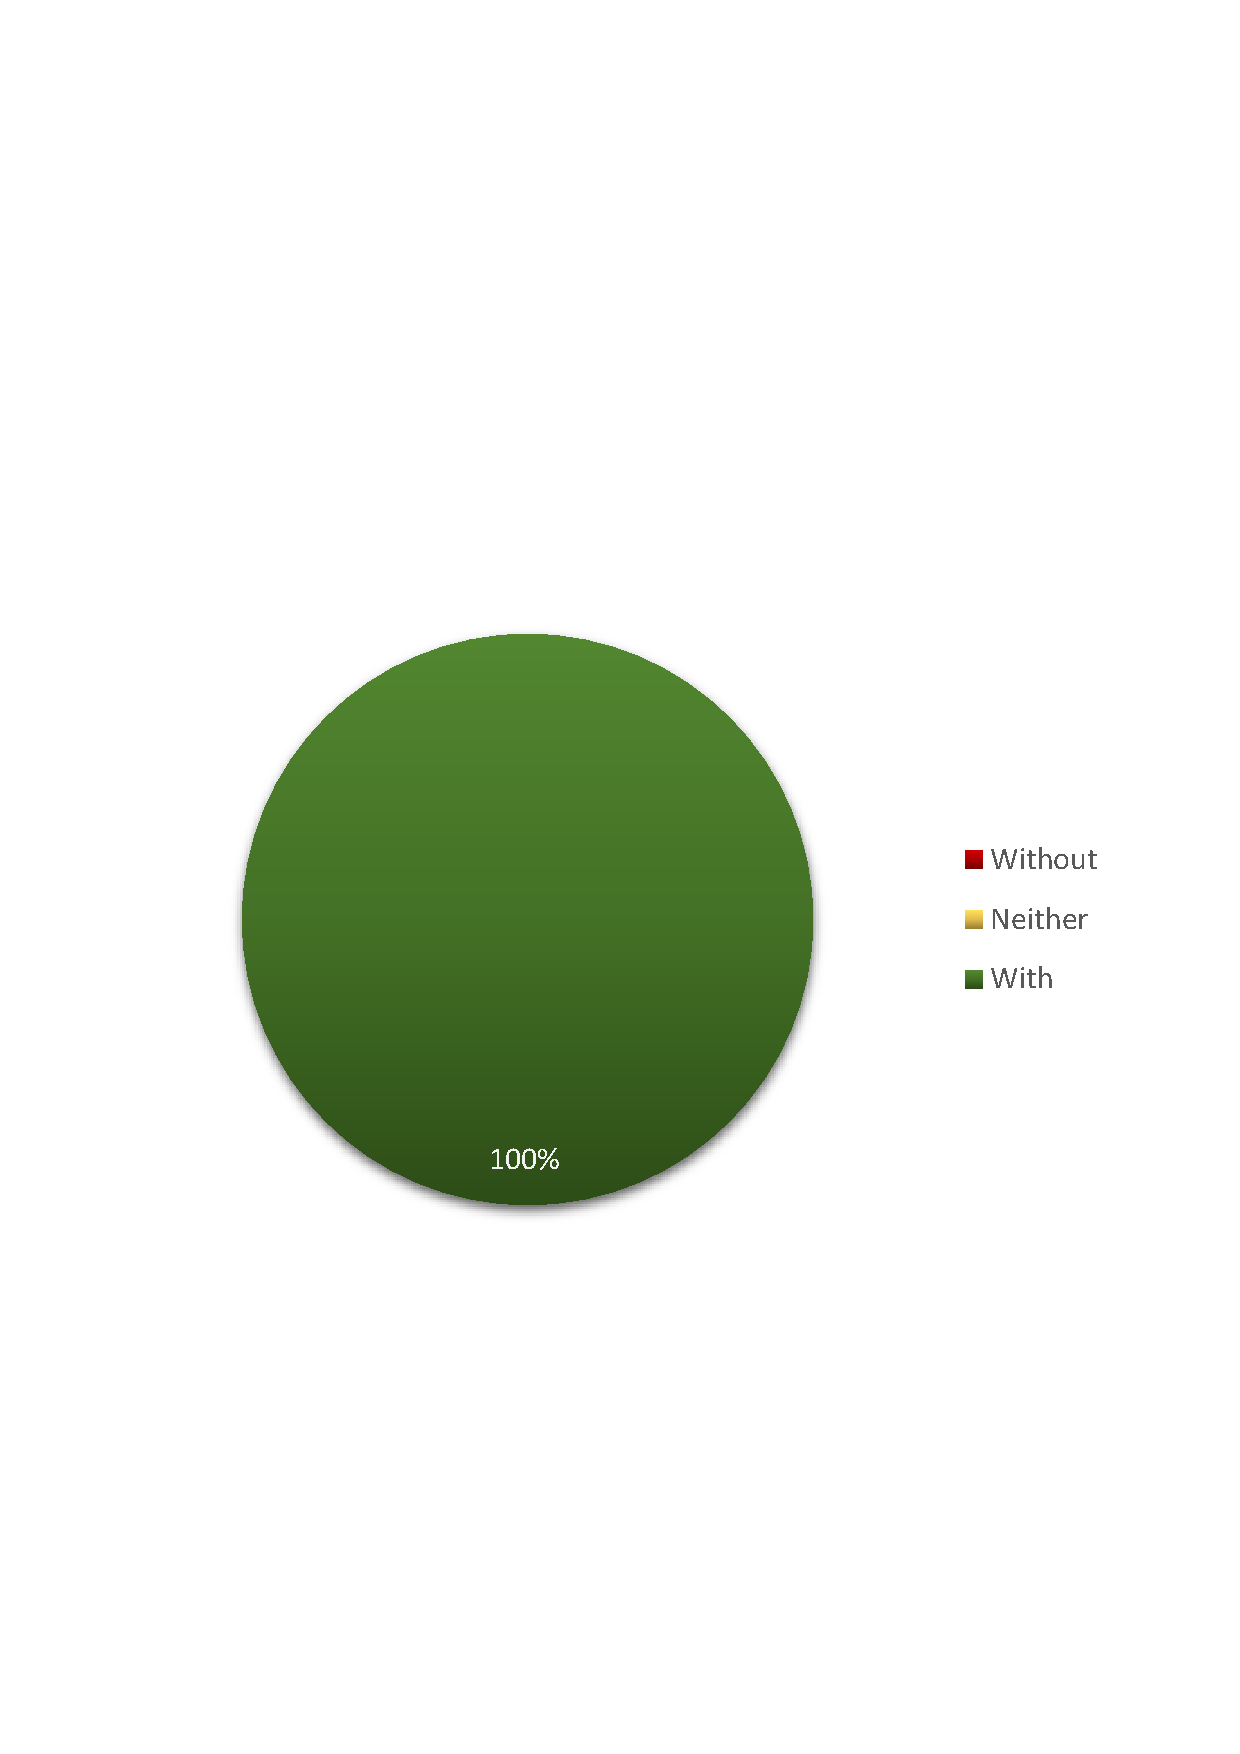
\includegraphics[width=0.6\textwidth]{images/charts/debugging_efficient.pdf}
	\caption{Efficiency of debugging}
	\label{fig:debugging_efficient}
\end{figure}

\begin{figure}[H]
  \centering
    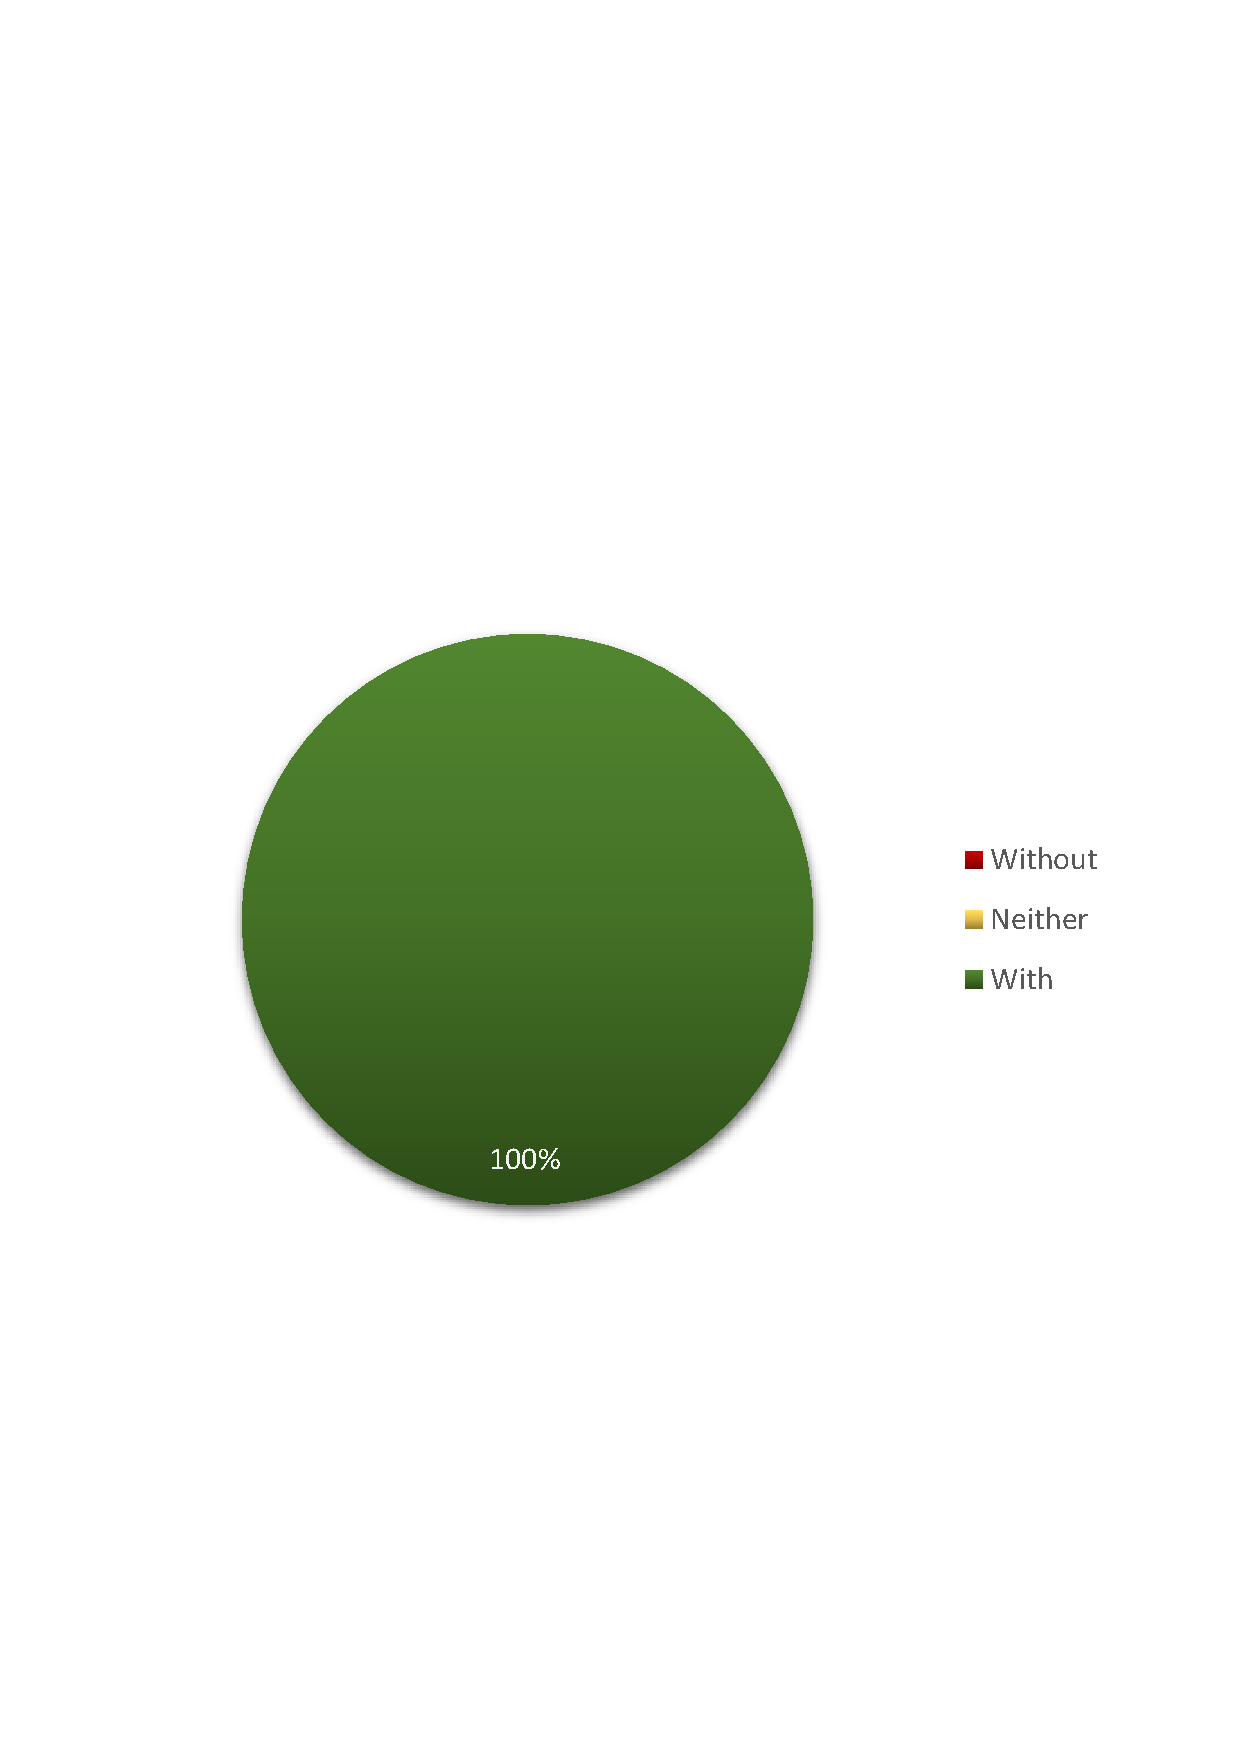
\includegraphics[width=0.6\textwidth]{images/charts/prefer_debugging.pdf}
	\caption{Preference for debugging}
	\label{fig:prefer_debugging}
\end{figure}


We also asked the participants if they would use our tools for debugging and implementing cross-device applications and if they think that our tools would be useful. The results can be seen in figure ~\ref{fig:usefulness_tool}. Almost all participants think that our tool would be very useful for implementing as well as debugging cross-device applications and the remaining few also think that they would be useful. All participants would use our tools for implementing cross-device applications and all except one participant would use them for debugging cross-device applications.

\begin{figure}[H]
  \centering
    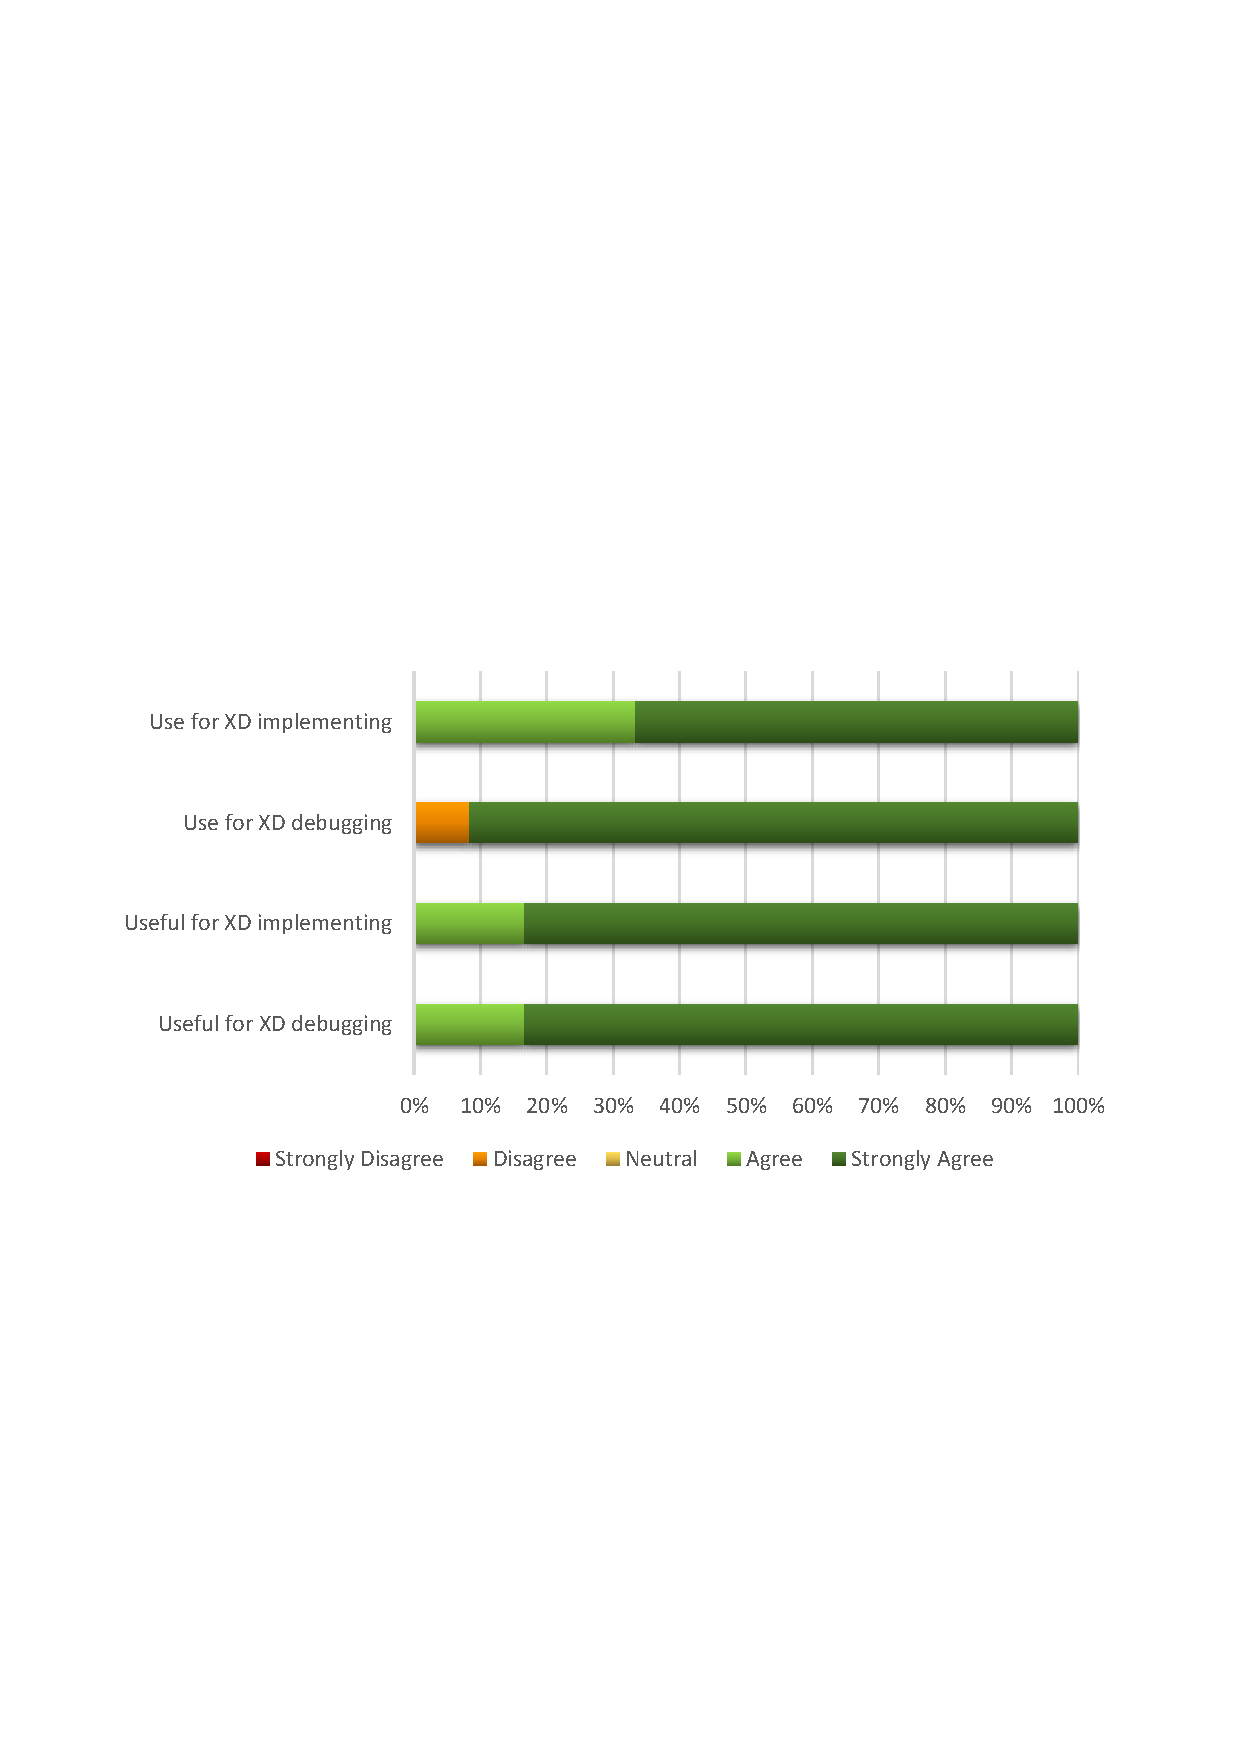
\includegraphics[width=0.8\textwidth]{images/charts/usefulness_tool.pdf}
	\caption{Usefulness of our tools}
	\label{fig:usefulness_tool}
\end{figure}

Finally, you can see the results for the general questions about our tools in Figure ~\ref{fig:tool_general}. The figure shows that our tools were perceived as easy to learn despite the many different features and the participants also felt rather confident using our tools. Our tools are not considered as unnecessarily complex at all. This indicates that the interface of our tools is generally well-structured and it would be easy for developers to get used to our tools.

\begin{figure}[H]
  \centering
    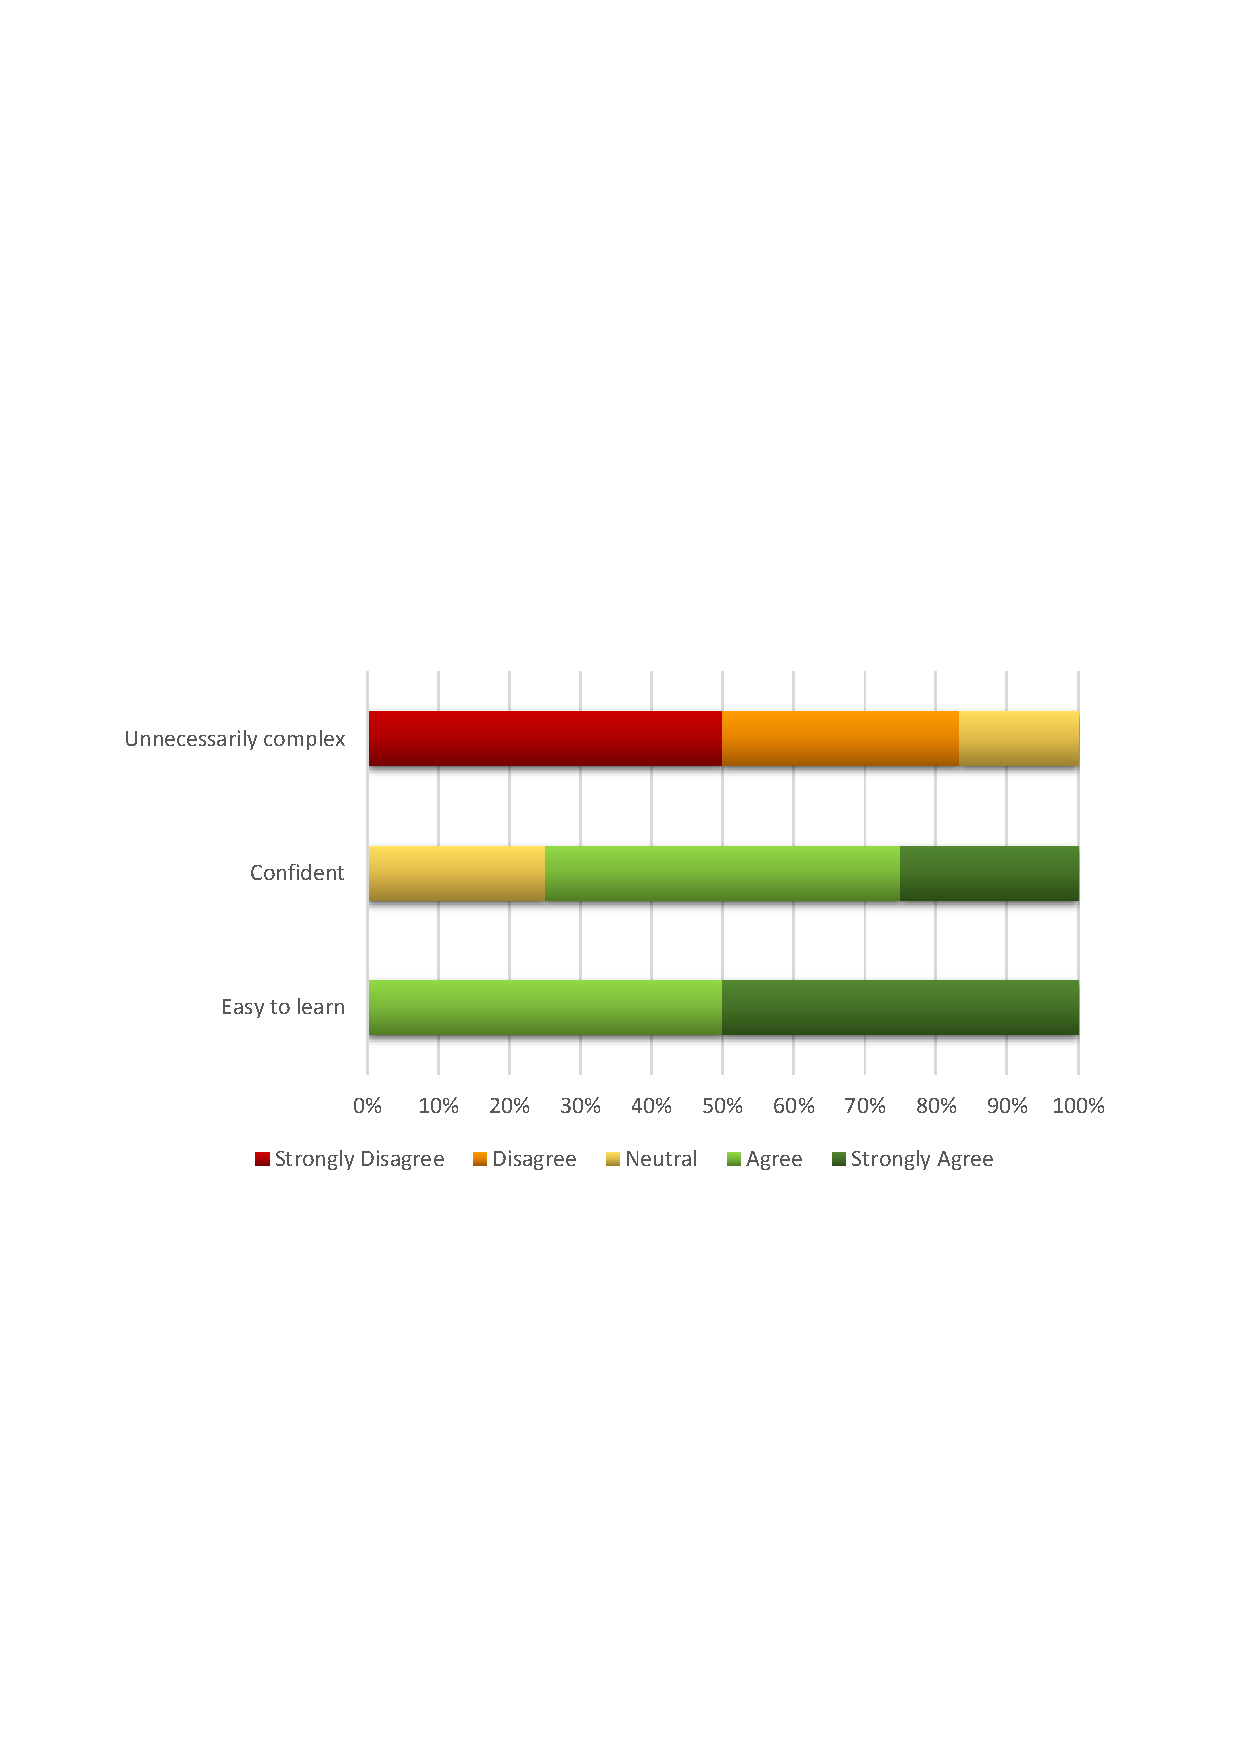
\includegraphics[width=0.8\textwidth]{images/charts/tool_general.pdf}
	\caption{General evaluation of our tools}
	\label{fig:tool_general}
\end{figure}

Figure ~\ref{fig:would_use_features} shows which features the participants would use for implementing and debugging cross-device applications. In general, people would rather use emulated devices rather than connecting real devices for both implementing and debugging. This is understandable as most things can be done just as well with emulated devices as with real devices. Some participants mentioned that they would not really use real devices during implementing, but that they would test their application on real devices after finishing implementing to make sure the application works fine on them. The connection features are almost unavoidable to use, thus it is surprising that some participants state that they would not use them. However, for some parts of debugging and implementing, one device might be sufficient for testing and no connection features would be required. One participant mentioned that the connection features seem very natural and that there is no point in asking about their usefulness because it is obvious that they are useful. This indicates that the feature was indeed greatly appreciated by some participants. The shared JavaScript console is equally popular for debugging and implementing and would be used by almost all participants. Function debugging is more popular for debugging than for implementing. This corresponds to the actual results of the study and has been elaborated before. Apart from connecting real devices, the shared CSS editor is the least popular. This may be due to the fact that browsers already have quite mature CSS editors and it might be possible to test CSS on one device at a time in many cases. Also, the CSS parts of our tasks were rather simply, thus the real value of such a feature might not be obvious to the participants. While things like changing the background color of a button can easily be done on just one device, more complex CSS problems like positioning elements require more effort and look much different on different devices.

\begin{figure}[H]
  \centering
    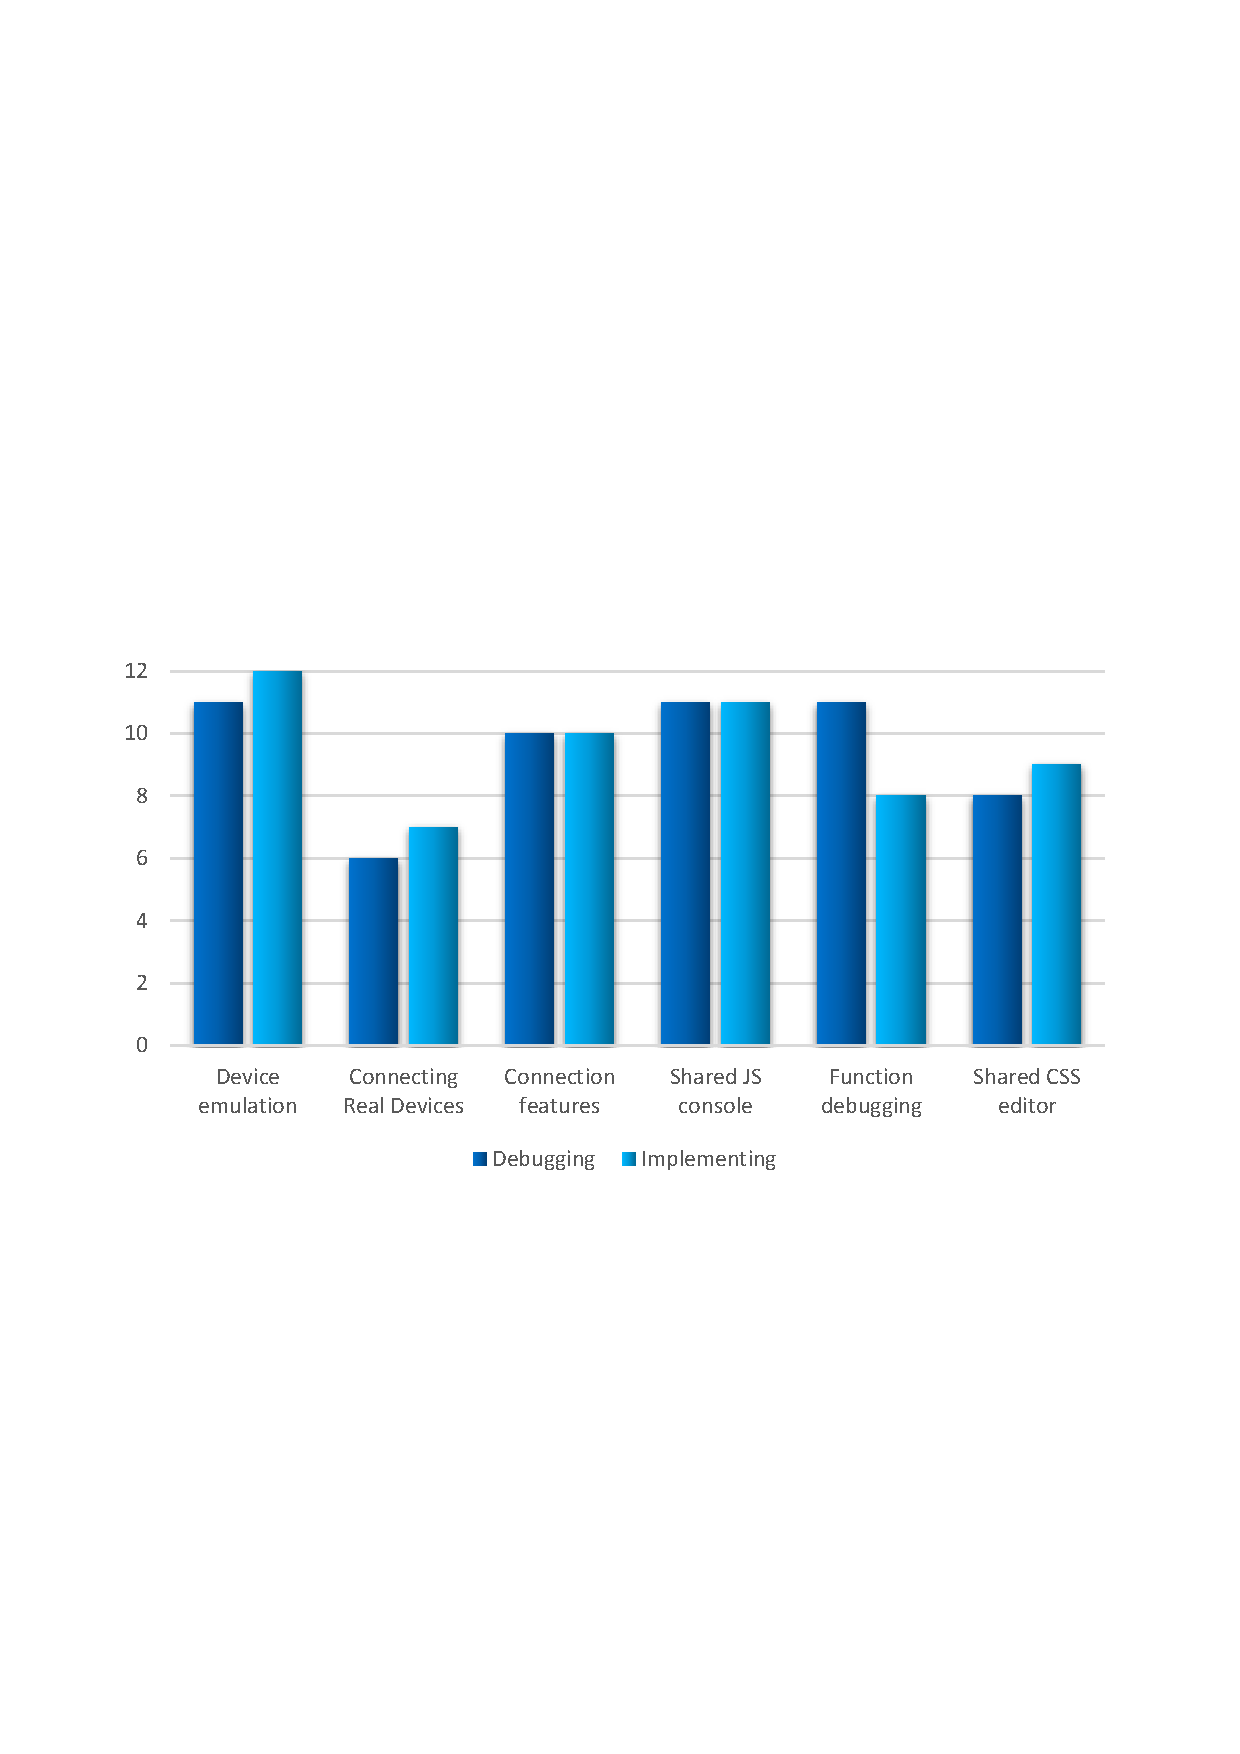
\includegraphics[width=0.8\textwidth]{images/charts/would_use_features.pdf}
	\caption{Features that the participants would use}
	\label{fig:would_use_features}
\end{figure}

During the study, some participants mentioned that they found device emulation very useful because they can have all devices in one place instead of having to manage different browser windows and profiles. Reloading all devices at once was also considered very useful. With multiple browser windows, each window has to be reloaded individually which makes this a much more tedious task. It was also appreciated that the devices are still connected after reloading, though this is also the case with multiple browser windows. The participants really liked function debugging, the only critique was that it does not show on which device a function is called which was fixed after the study. In general, the output aggregation of the shared JavaScript console was considered more useful than sending commands. One participant even mentioned that he would not use it to send commands, but the aggregation is very useful. 

Record/replay was disabled for the user study, but one participant that had attended a presentation about our tools before, mentioned that they would find it immensely useful. They consider it as a powerful feature that could be very helpful for replicating bugs in an application and for regression testing. Often, it is not clear how to reach a bug and being able to record the set of interactions that lead to the bug and then replay them can simplify this process.